\chapter{Experimental Methods}
\label{Chap:Methods}

The following Chapter introduces a selection of experimental methods and techniques relevant in the context of the experimental results presented in this thesis and other laser wakefield acceleration (LWFA) experiments. The three main ingredients of an LWFA experiment will be covered: a high-intensity laser, gas targetry and diagnostics for particles and secondary radiation. The measurement of high-energy gamma radiation will be discussed more extensively as it is central to this work.

The Chapter starts by introducing the \textsc{Gemini} laser system, the dual-beam high-intensity laser used to conduct the experiments in this work, along with diagnostics and methods to characterise high-intensity laser pulses.
It then continues with a section on gas targets and techniques to diagnose the plasma, followed by particle diagnostics.
Finally, the chapter focuses on diagnostics for high-energy radiation in the gamma regime, in particular a scintillator array used to infer gamma spectra.
A comprehensive review of diagnostics used in LWFA experiments is, for instance, provided in \cite{Downer2018_DiagnosticReview}.

\section{The Gemini laser system}

All experimental results presented in this work were acquired at Target Area 3 using the \textsc{Gemini} laser \cite{Hooker2006_Gemini,Hooker2008_Gemini} of the Central Laser Facility, Rutherford-Appleton Laboratory, UK.

\subsection{Laser properties}

The titanium-sapphire \textsc{Gemini} laser system provides two beams every 20 seconds at a compressed pulse duration of down to $30\,\mathrm{fs}$ and up to $15\,\mathrm{J}$ energy on each arm at a central wavelength of $800\,\mathrm{nm}$ \cite{GeminiWebsite}. The collimated beams that enter the target chamber have a diameter of just under $\sim 150\,\mathrm{mm}$, a flat-top intensity profile and are focused with a spherical mirror or off-axis parabolas (OAPs). Adaptive optics (AOs) are deployed on both laser arms in conjunction with wavefront sensors to remove aberrations and flatten the wavefront.
In addition to its full-power capabilities, a diode continuous-wave mode for alignment and a low power pulsed mode at 10 Hz repetition rate are available.

%\EliasComm{Vacuum compressors, gate valves. CPA. Separate laser and target area.}

%\subsection{Target Area 3}

%At \textsc{Gemini} the laser and the target area, called Target Area 3, are located in the same building but separate rooms.
%The target area 
%\EliasComm{Rough dimensions. Dimensions of vacuum chamber. Extension chambers. Lasers around the centre. Motivate dimensions. Bunker dimensions are $8 \times 8$ m and 1 m thick walls and 0.6 m concrete roof, along with lead shielding.}

\subsection{Beam line geometries}


\begin{figure}
\centering
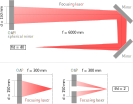
\includegraphics[width=0.8\columnwidth]{BeamGeometries.png}
\caption[Sketch of relevant focusing geometries used in experiments at \textsc{Gemini} discussed in this work.]{Sketch of relevant focusing geometries used in experiments at \textsc{Gemini} discussed in this work. Top: A long-focal-length geometry using an $f/40$ spherical mirror or off-axis parabola (OAP) used to drive a wakefield accelerator. Bottom: A short-focal-length $f/2$ geometry for a scatterer or heater beam using a full off-axis parabola (left) or an optic with a central hole (right).}
\label{Methods:Figs:FocusingGeometries}
\end{figure}
In the context of the LWFA experiments discussed later typically two types of beam line geometries are of relevance at \textsc{Gemini} (see Figure \ref{Methods:Figs:FocusingGeometries}):
First, a long-focal-length geometry using either an $f/40$ spherical mirror or an off-axis parabola with focal length $f = 6\,\mathrm{m}$ to provide an intense laser pulse with normalised vector potential $a_0 > 1$ and a long Rayleigh length, $z_R$, to efficiently drive LWFA over long distances. This geometry is used for the wakefield driver beam in all experiments discussed in this work. Due to the long focal length and the limited size of the target area and the vacuum chamber the beam has to be reflected or `folded' at least once during the focusing process, in recent setups about halfway between optic and focal plane (see Figure \ref{Methods:Figs:FocusingGeometries}, top). As a result, the maximum usable energy in this laser arm is limited by the damage threshold of these `folding' mirrors or in other words the fluence (optical energy delivered per unit area) the mirrors can sustain. The threshold at which damage occurs depends on several factors, including the beam quality and beam size, the quality of the mirror coating and cleanliness of the chamber.

The second focusing geometry is the short-focal-length scatterer (see Figure \ref{Methods:Figs:FocusingGeometries}, bottom) which is typically an $f/2$ off-axis parabola with focal length $f = 300\,\mathrm{mm}$. In the experiments discussed in Chapters \ref{Chap:linICS} and \ref{Chap:RR15} an off-axis parabola with a central fitted hole was used to enable a head-on counter-propagating geometry in conjunction with the long-focal-length beam line. 


\section{Laser Diagnostics}


\subsection{Laser Energy}
\label{Methods:Sec:LaserEnergy}

At \textsc{Gemini}, the laser energy is measured on every shot by collecting the laser light that is transmitted through the back of a highly-reflective dielectric mirror in the laser area and imaging it onto a CCD camera chip. The integrated number of counts on the CCD is calibrated using a laser energy meter (Gentec QE8SP-B-BL-D0) and the filtering is adjusted for different power modes.
A laser energy meter is also used to measure the reflectivity of the compressor gratings, at \textsc{Gemini} typically between 60 and 70 percent, and the energy reaching the interaction point (energy on-target).

\subsection{Laser Pulse Duration}
\label{Methods:Sec:PulseDuration}

At \textsc{Gemini}, frequency-resolved optical gating (FROG) \cite{FROG} is used to measure the pulse duration of the laser and characterise its temporal intensity profile.
A FROG trace is taken on every shot by collecting laser light that is transmitted through highly-reflective dielectric mirrors, similarly as for the on-shot energy measurement.

The FROG is a diagnostic to measure the intensity and spectral phase of ultrashort laser pulses as present at \textsc{Gemini} ($\sim 40\,\mathrm{fs}$). The setup is similar to an autocorrelator and is optically gated by combining two beams in a non-linear medium, typically a second-harmonic-generation crystal. The radiation is then spectrally resolved (hence frequency-resolved/\textit{FR}OG) and provides information about the spectral phase. See, for instance, \cite{FROG} and \cite{StreeterThesis} for more details.

\subsection{Focal Spot Characterisation}

The ability to characterise the properties of a focused laser pulse, in particular its size and peak intensity, is crucial for high-intensity laser experiments as it enables the optimisation of the focal spot shape for the respective application in an active feedback loop \cite{Gregory2015_f2OPT}, and also enables diagnosing the physical phenomena the laser is employed to probe or induce. In LWFA a short-pulse laser is focused down to reach high intensities to drive a wake, but has to guide itself over a long range at the same time. Only energy contained in the beam centroid is efficiently guided, whilst energy in the `wings' of the beam is lost and reduces the peak intensity of the laser pulse \cite{Mangles2012_SELF}. 
For Compton-backscatter experiments, on the other hand, a high intensity increases the yield of X-rays and is prerequisite to accessing nonlinear phenomena \cite{Corde2013_Rad}.
Since the energy in the laser pulses is limited and the temporal compression is also bounded (and not always desirable), the spatial shaping of the focal spot is a critical tool to reach efficiently high intensities.

A \textit{direct} measurement and characterisation of a high-intensity laser focus, also referred to as \textit{focal spot}, or even just its peak intensity is, however, very challenging.
For this reason, an attenuated low-power laser pulse is characterised instead at \textsc{Gemini}. In the low-power mode the laser pulses are amplified in all but the final amplification stage (see, for instance, \cite{PoderThesis} for more details on the laser beam line), propagate on the same beam path and through the same materials, and are manipulated by the same optics. As a result, the focal spot in the low-power and high-power mode are expected to be very similar, with exception of certain thermal effects.

At \textsc{Gemini} the low-power focal spot is imaged through a special long-working-distance microscope objective (Mitutoyo near-infrared infinity-corrected apochromatic) onto the CCD chip of an AVT Manta G-033B. To characterise the focal spot of the $f/40$ beam line (applicable to all experimental results) and the $f/2$ focal spot with phase plate (Chapter \ref{Chap:BW}) a microscope objective with magnification $\times10$ was used. A $\times20$ objective was used to image the focal spot from the $f/2$ beam line in the colliding-pulse experiments (Chapters \ref{Chap:linICS} and \ref{Chap:RR15}). A thin metal wire $ \sim 100 \microns$ was used to localise a well-defined spatial plane for the position of the focus, relative to which other components in the setup were then positioned. 

In order to produce an intensity profile of the laser pulse we require a measurement of the energy in the laser pulse, its temporal structure and spatial properties. The diagnostics for on-shot laser energy and pulse duration measurements were already presented in the previous section. The measurement of the spatial properties of the focal spot and how to relate the focal spot image to an intensity distribution is presented in the following.

\subsubsection{Spatial calibration}

The imaging system for the focal spot characterisation was spatially calibrated by imaging well defined line pairs on a transmissive resolution target, specifically a 1951 US Air Force Target (R1DS1P, Thorlabs). Figure \ref{Methods:Figs:FocalSpot_USAF} (left) shows an image of the central part of the USAF target, containing the smallest line pairs, with a sketch of the full USAF target pattern (negative) presented on its right side. A simple diode laser was used as backlighter. Each line pair is identified by its element and group number, and the related spatial dimension is given on the website of the manufacturer in units of line pairs per millimetre, lp/mm. By multiplying the size of a line pair on the image (pixels per line pair) with the dimensions given on the data sheet (line pairs per mm), we obtain the number of pixels corresponding to one millimetre or in inverse the size of one pixel, i.e. the spatial calibration of the image.
The magnification of the imaging system, $M$, on the other hand, is then simply the physical size of one camera pixel, which can be found on the datasheet of the camera in use, divided by the determined spatial scale that corresponds to one pixel on the image:
\begin{equation}
M = \frac{image\,pixel\,size\,[\mu m/ pxl]}{{camera\,pixel\,size\,[\mu m/pxll]}} = \frac{pixels\,per\,line\,pair/line\,pairs\,per\,mm}{{camera\,pixel\,size\,[\mu m]}}.
\end{equation}

Using the image shown in Figure \ref{Methods:Figs:FocalSpot_USAF} as an explicit example: One line pair of the second element of the 6th group measures 15 pixels. According to the data sheet this element has a scale of $71.8\,\mathrm{lp/mm}$, such that we obtain for the image $1077$ pixels/mm or $0.93 \microns$/pixel. The camera was of type AVT Manta G-033B with $9.9\microns$ physical pixel size, which then gives a magnification of $10.65$.

\begin{figure}
\centering
\includegraphics[height=0.35\columnwidth]{USAF_FocalCalib_Example.jpg}\includegraphics[height=0.35\columnwidth]{USAF_Resolution_Chart_A1-780.jpg}
\caption[Spatial calibration target for a focal spot camera.]{USAF targets to spatially calibrate the imaging system of the focal spot camera. Left: Central part of a transmissive USAF target backlit by a diode laser. Right: Full (negative) USAF pattern. The groups in the centre (numbers not legible) correspond to the groups shown on the left.}
\label{Methods:Figs:FocalSpot_USAF}
\end{figure}

\subsubsection{Intensity Distribution and Peak Intensity}
\begin{figure}
\centering
\includegraphics[width=0.33\columnwidth]{RRf40Spot.png}\includegraphics[width=0.33\columnwidth]{RRF2Spot.png}\includegraphics[width=0.33\columnwidth]{QEDPhasePlate.png}
\caption[Examples of low-power focal spots from different focusing geometries, measured at \textsc{Gemini}.]{Examples of low-power focal spots from different focusing geometries, measured at \textsc{Gemini}. The x- and y-axes show the horizontal and vertical spatial scale in micrometres, the colour scale shows the peak intensity in units of $W/cm^2$ on a linear scale (bottom row) and a logarithmic scale (top row). The focusing optics were an $f/40$ off-axis parabola (left column) and an $f/2$ off-axis parabola (central and right column). A phase plate was inserted into the collimated beam path of the laser pulse shown in the right column. The halo around this spot causes scattering in the imaging system which leads to the apparent rectangular region of intensity visible on the logarithmic scale (top) but is not a physical representation of the spot itself. The images were taken at \textsc{Gemini} in 2019 (left, centre) and 2018 (right).}
\label{Methods:Figs:FocalSpotExamples}
\end{figure}

The image of the low-power focal spot on the CCD is a temporally integrated measurement of the profile of the laser pulse. Given an appropriate background subtraction, no saturation on the image and given that the entire focal spot is captured on the image, the total pixel count corresponds to the total energy in the laser pulse and the distribution of the counts in turn corresponds to the spatial energy distribution. This also applies to the high-power focal spot as we assume that the low-power laser pulse is representative of the high-power pulse. By relating the on-shot energy measurement (see Section \ref{Methods:Sec:LaserEnergy}) to the total pixel count on the image we obtain an energy calibration in units of $J/pixel\,counts$. Since the image is spatially calibrated, we can assign each pixel in turn a fluence, $pixel\,counts/area \rightarrow J/area$. If we now fold in the time over which this fluence is delivered, we obtain the intensity, energy per unit time and area, here given in the units $\mathrm{W/cm^2}$. By considering the entire pulse duration (see Section \ref{Methods:Sec:PulseDuration}) this corresponds to the average intensity. If we extract the peak power from the pulse envelope (FROG trace), we can determine the peak intensity, which is the driving quantity in most LWFA and colliding-pulse experiments.
Finally, as a result, we obtain the spatial distribution of the peak intensity of the focal spot. 

Using the methods described in this section the intensity distributions for three example focal spots from different focusing geometries were calculated and are shown in Figure \ref{Methods:Figs:FocalSpotExamples} (note different spatial scales), where the colour scale indicates the intensity in $\mathrm{W/cm^2}$. The top and bottom row show the same focal spots but on a logarithmic scale (top) and a linear scale (bottom), respectively. The laser pulses were focused by an $f/40$ off-axis parabola (left column) and an $f/2$ off-axis parabola (centre and right). A phase plate \cite{Kato1984_PHASEPLATE} was inserted into the collimated beam to obtain the wide, speckled focal spot on the right, which was used as X-ray heater beam in the experiment described in Chapter \ref{Chap:BW}. The other two focal spots were measured on a \textsc{Gemini} campaign in 2019 (Chapter \ref{Chap:linICS}).





\section{Dual-Beam Timing Diagnostics}
\label{Methods:Sec:DualBeamTiming}

 
All of the experiments discussed in this thesis use both laser arms of \textsc{Gemini}, so that their laser pulses have to be overlapped in space and synchronised in time, or in other words they have to be `timed' to each other. This section discusses the two diagnostics, photodiodes and (spatial) interference, that were used to measure the temporal separation of the two laser pulses. Photodiodes were employed to measure and account for relatively `large' separations on the nanosecond to few picosecond level, which was by itself sufficient for the experimental setup described in Chapter \ref{Chap:BW}. The colliding-pulse experiments described in Chapters \ref{Chap:linICS} and \ref{Chap:RR15}, on the other hand, required a femtosecond level synchronisation of the laser pulses, for which interference occurring between them within the time scale of their pulse envelopes was used in addition. Two plane waves crossing at an angle produce an interference pattern of parallel straight lines, whereas a plane wave interfering with a spherical wave front results in a circular pattern. Two laser pulses that expand at different f-numbers, here $f/2$ and $f/40$, behave similarly as the latter case as the radii of curvature of their wave fronts differ strongly. The presence of a circular interference pattern then signals temporal overlap within their combined pulse duration at an accuracy of tens of femtoseconds.
At the end of this section the implications for electron-laser timing from a perspective of laser-laser timing, and effects from other experimental procedures specific to \textsc{Gemini}, such as the pump-down of the vacuum chamber or the attenuation of the laser pulses, are considered.

At \textsc{Gemini} both laser arms are `intrinsically' synchronised as they originate from the same source (oscillator), but might arrive at the interaction point at different times as they travel on different beam paths. By measuring the difference in the time of arrival of both laser pulses, $\Delta \tau$, the length of the beam paths can be adjusted accordingly, such that $\Delta \tau \rightarrow 0$, i.e. the laser pulses are `timed'. Temporal separations on the nanosecond level are typically corrected by extending the beam path of the `early' laser pulse by several optics. Smaller adjustments corresponding to temporal shifts of tens of picoseconds or less are performed using a motorised linear stage (Newport M-ILS250) on the `split-and-delay' (SAD) table in the laser area. The SAD delay stage adds or removes beam path in double-pass at micrometre or correspondingly few femtosecond precision.

\subsection{Photodiodes}
\label{Methods:Sec:DiodeTiming}

In the experiments described in this thesis two attenuated (low power) laser pulses were spatially overlapped at the interaction point. The pulses are then either directed onto the active chip of a photodiode or are scattered from an object placed at the interaction point, for instance a piece of lens tissue, which the photodiode then faces. Each laser pulse triggers a response in the photodiode that can be measured with an oscilloscope. Since each pulse is only $\sim 40\fs$ long, almost instantaneous for the diode, the response for each pulse is a symmetric peak with the rise/fall time as width. The relative time of arrival can then be determined by measuring the separation of the two peaks. At \textsc{Gemini} the fast EOT-4000 GaAs photodetector (see Figure \ref{Methods:Figs:Photodiode}) with a rise/fall time of $< 30\,\mathrm{ps}$ was used in conjunction with a Lecroy WaveMaster 813Zi-B oscilloscope ($>13\,\mathrm{GHz}$). The detectors were only used in air and were not tested for vacuum use.


\begin{figure}
\centering
\includegraphics[height=0.38\columnwidth]{PhotoDiode_BW.jpg}\includegraphics[trim={2.0cm 0 2cm 0}, clip, height=0.38\columnwidth]{DeadReckonDiode.png}
\caption[Photo of a photodiode used in experiment and timing scan using a delay stage and a photodiode.]{Left: Photodiode (black) used in the experiments in this work (EOT-4000 GaAs). The active area is inside the round `window'. The white strip is used to scatter the laser and increase the signal yield. Right: Temporal separation between two laser pulses ($f/40$ and $f/2$) measured with a fast diode and oscilloscope. The plot shows how much earlier the $f/40$ laser pulse arrives as a function of the position of the delay stage (SAD position). In the region between 15 and 40 picoseconds the peaks start to merge and measurement of the separation becomes unreliable. The linear fit can be used to identify the delay required to match the time of arrival of both laser pulses. The shaded region indicates the 95 percent confidence interval for the fit.}
\label{Methods:Figs:Photodiode}
\end{figure}


Photodiodes and oscilloscopes are relatively straightforward to set up and use, but due to their typical rise/fall time of several tens of picoseconds the accuracy of an individual measurement using an appropriate oscilloscope is $\sim10\,\mathrm{ps}$. The accuracy of the synchronisation can be improved by conducting multiple measurements across a range of relative temporal delays and then interpolating between the data points to obtain the zero-delay point. At \textsc{Gemini} the delay stage on the SAD table can be moved to adjust the relative delay of both laser arms. Since the stage moves at micrometre precision the main experimental error for each measurement is the reading error on the oscilloscope. 

The result of such a scan in relative delay is shown in Figure \ref{Methods:Figs:Photodiode} (right) for data taken on the experimental campaign presented in Chapter \ref{Chap:linICS}: the relative delay of the two laser pulses (here in terms of how much earlier the $f/40$ laser pulse arrives) as measured with the photodiode and the oscilloscope is shown as a function of the SAD position. When both pulses arrive within each other's rise or fall time the diode responses merge and the peaks can not be properly distinguished, which is why there are no data points around the zero-delay point. The linear fit to the data points is parametrised by $y_{fit} = 6.78 \,[\mathrm{ps/mm}]\, \times\,x_{SAD}[\mathrm{mm}] - 178.72\,[\mathrm{ps}]$ which indicates that the zero point is at $x_0 = (26.36 \,\pm\, 0.68)\mm$. The error on the SAD position (equivalent to $\sim 2\,\mathrm{ps}$) was estimated using the $95\%$ confidence interval of the linear fit (shaded area in Figure \ref{Methods:Figs:Photodiode}).

\subsection{Interferometry}
\label{Methods:Sec:SpatialInterferometry}

Diode timing as described in the previous section can measure up to nanosecond temporal separations but is limited to an accuracy of a few picoseconds. It is a suitable technique to `roughly' synchronise the two laser pulses. Interference of the two laser pulses can be used to synchronise the two laser pulses to the femtosecond level.


Considering the electric fields of two plane waves with the identical frequency $\omega$ and polarisation but different wave vectors $\mathbf{k_1}$, $\mathbf{k_2}$, time of arrival $t_1$, $t_2$ and initial phase $\phi_1$, $\phi_2$ can be written as:
\begin{equation}
\mathbf{E_1} (\mathbf{r},t_1) = E_1 e^{i(\omega t_1 - \mathbf{k_1} \cdot \mathbf{r} + \phi_1)} \mathbf{e_x},\,\, \mathbf{E_2} (\mathbf{r},t_2) = E_2 e^{i(\omega t_2 - \mathbf{k_2} \cdot \mathbf{r}+\phi_2)} \mathbf{e_x},
\end{equation}
where $\mathbf{e_x}$ is a unit vector indicating the polarisation, $\mathbf{r}$ is the position vector and $E_1, E_2$ are the amplitudes of the electric fields.
The combined intensity of both plane waves, for instance at the plane of the detector, is 
\begin{equation}
I = \frac{1}{4}\epsilon_0 \mathbf{E} \cdot \mathbf{E}^\ast, 
\end{equation}
where $\mathbf{E}^\ast$ is the complex conjugate of $\mathbf{E}$, and $\mathbf{E} = \mathbf{E_1} + \mathbf{E_2}$, or more specifically
\begin{equation}
I = \frac{\epsilon_0}{4}\left|E^2_1 + E^2_2+ E_1 E_2 \cos(2 ky \sin\theta - \omega \Delta \tau + \Delta\phi )\right|,
\end{equation}
where $\theta$ is the angle between the two plane waves, $\Delta \tau$ the difference in their time of arrival and $\Delta \phi$ the difference in the initial constant phase. The relation shows that the crossing plane waves produce a straight interference pattern due to the angle, $\theta$, between them which vanishes when both wave vectors are parallel, i.e. $\theta = 0$. The contrast, the difference between the maxima and minima $(I_{max} - I_{min})/(I_{max} + I_{min})$, is optimised for equal field amplitudes, $E_1 = E_2$. 
If we consider a plane wave and a spherical wave instead, the resulting interference pattern will produce concentric rings due to the radius of curvature:
\begin{equation}
I \sim 1 + \cos\left(\frac{\pi r^2}{\lambda R}\right),
\end{equation}
where we simplified the relation by assuming that the wave vectors are parallel and $\Delta \tau = 0,\,\Delta \phi = 0$, i.e. in contrast to the previous case the interference pattern does not vanish for parallel waves. In the limit of $R \rightarrow \infty$ this approaches the case of two plane waves. 

A focusing and defocusing Gaussian laser pulse changes its radius of curvature, $R$, where the wave front is strongly curved near the focus (within few Rayleigh lengths, $z_R$), especially for tightly focused beams, and asymptotically flat at a distance $|z| \gg z_R$ away from the focus or weakly focused beams (see Section \ref{Chap:Theory:Sec:LaserInVac}). As a consequence, one can produce straight or circular fringes by interacting two Gaussian laser pulses either close or far away from their foci, or by focusing one with a low f-number and the other one with a high f-number optic.
\vspace{\baselineskip}


Ultrashort laser pulses require large bandwidths, $\Delta f$, such that the coherence length, $l_{coh}$, is very short ($l_{coh} \propto 1/\Delta f$), here comparable to the pulse duration. As a result, the variation in the interference pattern due to a change in the term $\omega \Delta \tau$ can be neglected when varying the relative delay between two pulses. The interference pattern only appears when both pulses arrive at the detector plane within the limited time window of their combined pulse durations with an optimised contrast of the pattern when the beams are centred on each other in space and time as then the entirety of the pulses interfere. This method is here referred to as \textit{spatial interferometry}. Since the `active' time window in which the pattern appears is very small an initial `rough' timing using the photodiodes described in the previous section is of advantage.

On the other hand, it is possible to increase the coherence length by dispersing both laser pulses with a grating such that the individual frequency components interact separately, assuming both pulses are identically chirped. This method is referred to as \textit{spectral interferometry}. See for instance \cite{Corvan2016_TIMING} for a detailed description. Depending on the dispersion this enables an active window of hundreds of picoseconds and in turn allows using the variation of $\omega \Delta \tau$ to quantitatively determine the temporal separation of the laser pulses as it is now encoded in the wavelength of the interference pattern.

\subsubsection{Experimental Implementation}
\begin{figure}
\centering
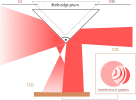
\includegraphics[height=0.35\columnwidth]{PrismCam.png}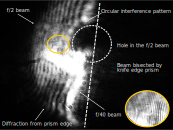
\includegraphics[height=0.35\columnwidth]{PrismCamExample.pdf}
\caption[Realising spatial interferometry as timing diagnostic in an experiment (sketch and example from an experiment).]{Realising spatial interferometry as timing diagnostic in an experiment. Left: Sketch of a spatial interferometry setup used in the experiments described in this work. Two counterpropagating laser beams are reflected collinearly from a 90-degree knife-edge prism and onto a CCD (brown). One laser pulse is highly divergent ($f/2$, left), the other one has a comparatively long Rayleigh length ($f/40$, right). The different radii of curvature result in a circular interference pattern when both laser pulses are overlapped in space and time. The prism can be translated to only reflect half of each beam (dotted prism). Right: Example of spatial interferometry (circular interference pattern) measured in an experiment using a setup as sketched out on the left with an attenuated (low-power) pulsed $f/2$ (OAP with hole) and an $f/40$ beam. Both beams aligned such they are effectively bisected by the knife-edge prism (spatial overlap, see dotted prism in the sketch on the left). As a result the $f/2$ beam shows straight diffraction patterns in its near field. The hole in the $f/2$ beam is also clearly visible and the circular interference pattern is centred on it which indicates that both beams are close to parallel and the interference pattern mainly originates from the different radii of curvature.}
\label{Methods:Figs:PrismCamSketchPlusExample}
\end{figure}


In the experiments discussed in Chapters \ref{Chap:linICS} and \ref{Chap:RR15} spatial interferometry was used to synchronise two counterpropagating laser pulses of pulse duration $\sim 45\fs$, one focused by an $f/2$ off-axis parabola (OAP), the other by an $f/40$ OAP or spherical mirror. The laser pulses are cross-polarised and the timing measurements were performed in an attenuated low-power mode. To combine both beams a 90-degree reflective knife-edge prism (Thorlabs, protected aluminium/dielectric) was placed at the interaction point, which reflects the counterpropagating beams collinearly onto the CCD chip of a camera (see Figure \ref{Methods:Figs:PrismCamSketchPlusExample}, left).
By gradually translating the prism away from the CCD the two laser beams move closer to the knife edge of the prism and in the process closer together until only one half of each beam is reflected  (see dotted prism outline in Figure \ref{Methods:Figs:PrismCamSketchPlusExample}, left). By now moving the CCD in the opposite direction the beams diverge and overlap with each other: we achieved spatial overlap. When both pulses are also synchronised in time a circular interference pattern will appear which allows a synchronisation of both beams to about $\sim 30\fs$. An example of this final configuration from the experiment described in Chapter \ref{Chap:linICS} is shown in Figure \ref{Methods:Figs:PrismCamSketchPlusExample} (right), where the large half circle with the central hole is the divergent $f/2$ laser pulse and the bright spot is the $f/40$ beam that expands only slowly. The straight, vertical interference pattern is due to diffraction from the knife edge, whereas the circular, more closely spaced circular pattern results from the interference between both two pulses.

\begin{figure}
\centering
\includegraphics[height=0.4\columnwidth]{FringeVisibilityCole.png}
\caption[Visibility of the interference pattern (fringes) as a function of the relative delay from a reference position.]{Visibility of the interference pattern (fringes) as a function of the relative delay from a reference position for data taken on an experimental campaign at \textsc{Gemini} in 2015. Figure courtesy of J. Cole (Imperial College). }
\label{Methods:Figs:PrismCam_FringeVisibility}
\end{figure}

The camera was equipped with a long-working-distance microscope objective ($\times 10$ Mitutoyo Plan Apochromat Near-Infrared) and a linear polariser.
The polariser is prerequisite for interference but was also be used to adjust the relative brightness of both beams to increase the contrast of the interference pattern. The contrast was also adjusted by taking advantage of the different divergences of the beam and moving the imaging plane closer or further away from the focus.
Once the contrast was maximised the visibility of the pattern was optimised to determine the temporal overlap more accurately. The accuracy of the synchronisation can be improved through statistical measurements, similarly as described for the diode timing. In Figure \ref{Methods:Figs:PrismCam_FringeVisibility} the `fringe' (interference pattern) visibility is shown as a function of the SAD position, using data analysed for \cite{Cole2018_RR} by J. Cole (Imperial College). The position for the optimum overlap was determined through a fitting routine. The uncertainty of this technique was estimated to be $\sim 17\fs$.

\subsection{Additional considerations for the synchronisation of beams}

The synchronisation of two laser pulses to each other or of a laser pulse with an electron beam to the femtosecond level is very challenging (even if we neglect the spatial overlap to the micrometre level). In this section we will discuss certain factors that had to be considered in the context of the experiments at \textsc{Gemini} discussed later in this thesis as they affected the timing procedure.

One key reason is the fact that light moves slower through media than through vacuum. The group velocity, $v_g$, is reduced by the refractive index, $\eta$, to $v_g =c/\eta$ or more specifically in a plasma to $v_g \approx c(1-1/2 (\omega_p/\omega)^2)$ (see Section \ref{Theory:Sec:LaserPropagationPlasma}), where $\omega$ is the frequency of the laser and $\omega_p$ is the plasma frequency (see Section \ref{Chap:Theory:Sec:PlasmaFreq}).
Introducing or removing media asymmetrically from beam paths changes the relative time of arrival of the laser pulses.
Typical examples at \textsc{Gemini} for this are moving from air to vacuum (pumping down the vacuum chamber), opening or closing the transparent gate valves, or attenuating beams using glass slides when switching between different power modes.

\subsubsection{Shifting beam paths from air to vacuum}

The refractive index of vacuum is $\eta_0 = 1$, whereas the refractive index of air, for instance, at $20^\circ$ Celsius, $45\%$ relative humidity and atmospheric pressure is $\eta_{air} = 1.00027$ for light of wavelength $\lambda = 800\,\mathrm{nm}$ \cite{Stone2011_ETAAIR}. The difference in time, $\Delta t$, it takes a laser pulse to travel a distance $d$ in vacuum or air is then proportional to the difference in the refractive indices:
\begin{align}
\Delta t &= \frac{d}{c} \left( \eta_{air} - \eta_{0}\right),\nonumber\\
\Delta t  &\approx 0.9\,\mathrm{ps} \times \frac{d}{1\,\mathrm{m}},
\end{align}
which means that it takes the laser pulse $0.9\,\mathrm{ps}$ longer to travel one metre in air than in vacuum.
If the beam paths of two laser pulses are of different length, the difference in their beam path will result in a shift in the relative time of arrival at the interaction point when transitioning from air to vacuum.

At \textsc{Gemini} the laser arm used as wakefield driver typically covers a beam path of over $10\,\mathrm{m}$ distance due to the long-focal-length geometry with $f = 6\,\mathrm{m}$, whilst the scatterer beam only covers about half of the distance. If both beams arrive at the same time at the interaction point when the chamber is at air, then a difference in $5\,\mathrm{m}$, for instance, would mean that in vacuum the laser pulse following the long-focal-length beam line arrives at the interaction point $4.5\,\mathrm{ps}$ after the scatterer.
\vspace{\baselineskip}

As a result of the pump-down process the components in the vacuum chamber and the vacuum chamber itself experience changes in pressure and temperature which in turn result in stress on the materials. This can lead to a steering of the laser beams which affects the alignment in general but also modifies the beam path.

\subsubsection{Opening and closing gate valves}

Another step in the pump-down process at \textsc{Gemini} is opening the transparent gate valves that separate the target chamber, which is often at air or lower quality vacuum, from the relatively permanent and high quality vacuum of the two laser compressors.
Once the pressure in the target chamber reaches a sufficiently low value and the turbo pumps are engaged, the gate valves can be opened.
Both gate valves at \textsc{Gemini} are made of sapphire glass, but measurements found a slight difference in thickness of around $\Delta x = 60 \pm 3\,\mathrm{\upmu m}$ \cite{GEMINI_GATEVALVES} corresponding to $\Delta t = 350\pm17\,\mathrm{fs}$ at a wavelength of $\lambda = 800\nm$. The gate valve of the laser arm that is predominantly used as wakefield driver was found to be thicker.

\subsubsection{Attenuation of beams}

The previous two examples can be cross-checked by repeating some of the timing procedures after the pump-down, for instance using again spatial interferometry, whereas the following example can not.
At \textsc{Gemini} glass slides are used as beam attenuators in the low-power modes and can be used in conjunction with polarisers and waveplates to improve the contrast of the interference pattern in spatial interferometry (see Section \ref{Methods:Sec:SpatialInterferometry}). In some cases this will require inserting material asymmetrically in both laser arms in order to optimise the visibility of the pattern.

The attenuators are $2\,\mathrm{mm}$ thick fused silica glass slides with refractive index $\eta = 1.4533$ \cite{Malitson1965_FusedSilica}. The slides are inserted at 45 degrees angle relative to the laser beam axis which delays the laser pulse by $4.24\,\mathrm{ps}$ for each glass slide. The attenuators were found to be identical to each other to within $\Delta x < 10\microns$, such that an equal number of attenuators in each beam path does not introduce a measurable relative delay. An unequal number of attenuators in each beam, on the other hand, requires an adjustment of the beam paths relative to the configuration at which the interference pattern is observed.

\subsubsection{Synchronisation of an LWFA electron beam with a laser pulse}
\label{Methods:Sec:Beam_Laser_Timing}

Using spatial interferometry the two laser pulses can be synchronised in vacuum to an estimated accuracy of $30\,\mathrm{fs}$. This timing is only valid if both laser pulses travel through vacuum. In a shooting scenario, however, the driving laser pulse propagates through plasma to accelerate electrons via LWFA. The propagation in a medium reduces the group velocity of the laser pulse and delays its arrival relative to the vacuum timing.
In the colliding-pulse experiments discussed in Chapters \ref{Chap:linICS} and \ref{Chap:RR15} we are in addition trying to overlap the scattering beam with the electrons accelerated by the driver pulse rather than the driver itself. The LWFA electron bunch trails behind the driving laser pulse and arrives later at the interaction point. Since the scattering beam arrives before both at its focal plane and the designated interaction point, the real collision will occur beyond this point. This is illustrated in a sketch in Figure \ref{Methods:Figs:LaserElectronOffset_Sketch}.
\vspace{\baselineskip}

\begin{figure}
\centering
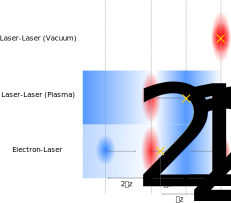
\includegraphics[width=0.8\columnwidth]{LaserElectronOffset_Sketch.png}
\caption[Sketch of two counterpropagating laser pulses and how the interaction point shifts in different scenarios.]{Top row: Two counterpropagating laser pulses (red) are synchronised to each other in vacuum so that they meet at a designated interaction point (yellow cross) $z = 0$ at $t = 0$. Central row: The laser pulse entering the sketch from the left now propagates through plasma and is slowed down such that at $t=0$ it is a distance $2\delta z_1$ separated from the designated interaction point (see Eqn. \eqref{Methods:Eqns:BeamLaser_Timing_deltaz1}). The laser pulses then meet halfway at $z = \delta z_1$ (yellow cross). Bottom row: An LWFA electron bunch is trailing behind the laser pulse at $2 \delta z_2$ distance (see Eqn. \eqref{Methods:Eqns:BeamLaser_Timing_deltaz2}). The effective interaction point is now at $\delta z = \delta z_1 + \delta z_2$ (see Eqn. \eqref{Methods:Eqns:BeamLaser_Timing_deltaz}).}
\label{Methods:Figs:LaserElectronOffset_Sketch}
\end{figure}

The following analysis explicitly derives Equation 2 in \cite{Cole2018_RR} and is based on work by Jason Cole (Imperial College).
We assume that the laser pulse travels through a plasma of electron density $n_e$ at the standard non-linear group velocity reduced by the etching velocity, $v_f \approx 1-\frac{3}{2}\frac{n_e}{n_c}$ (called front velocity in \cite{Decker1996_FV}), where $n_c$ is the critical density. Given a plasma of thickness $d$ the laser pulse of the scattering beam travels in the same time a distance  $d'=d c/v_f > d$.
Both laser pulses now meet at a distance $\delta z_1$ past the focal plane of the scattering beam (see Figure \ref{Methods:Figs:LaserElectronOffset_Sketch}, central row):
\begin{equation}
\delta z_1 = \frac{1}{2} \left[d \frac{c}{v_f} - d\right] = \frac{d}{2} \left[\left(1-\frac{3}{2} \frac{n_e}{n_c}\right)^{-1} -1\right] \approx \frac{d}{2}\left(1+\frac{3}{2} \frac{n_e}{n_c} -1\right) = \frac{3d}{4}\frac{n_e}{n_c}.
\label{Methods:Eqns:BeamLaser_Timing_deltaz1}
\end{equation} 



\begin{figure}
\centering
\includegraphics[width=0.8\columnwidth]{LaserElectronOffset.png}
\caption[Temporal offset between the laser pulse (in vacuum) and the electron beam, $\Delta \tau$, as a function of the injection point relative to the start of the plasma.]{Temporal offset between the laser pulse (in vacuum) and the electron beam, $\Delta \tau$, as a function of the injection point relative to the start of the plasma, $d$, for the dephasing limited case, $N = 1/2$, for different electron densities, $n_e$. The dashed lines indicate the delay $\Delta \tau$ for $d = 0$ for the respective electron density in the same colour.}
\label{Methods:Figs:LaserElectronOffset_ne}
\end{figure}


The electrons in turn trail around $N$ plasma wavelengths, $\lambda_p$, behind the driving laser pulse and meet the scattering pulse midway (see Figure \ref{Methods:Figs:LaserElectronOffset_Sketch}, bottom row):
\begin{equation}
\delta z_2 = \frac{1}{2} N \lambda_p = \frac{1}{2} N \frac{2 \pi c}{\omega_p} = \frac{1}{2} N \frac{2 \pi c}{\omega} \frac{\omega}{\omega_p} = N \frac{\lambda_0}{2} \sqrt{\frac{n_c}{n_e}}.
\label{Methods:Eqns:BeamLaser_Timing_deltaz2}
\end{equation}
The smallest possible value of $N$, assuming a homogeneous plasma, is $N = 1/2$ which is when the acceleration is close to its dephasing limit.
Under these assumptions the electron bunch and the scattering beam meet at $\delta z$ distance from the intended collision point:
\begin{equation}
\boxed{\delta z = \frac{3d}{4} \frac{n_e}{n_c} + N \frac{\lambda_0}{2}\sqrt{\frac{n_c}{n_e}},}
\label{Methods:Eqns:BeamLaser_Timing_deltaz}
\end{equation}
where in this context $d$ is the distance of the injection point from the front of the plasma. We can instead also determine, similarly as before, the temporal offset, $\Delta \tau$, relative to the vacuum laser-laser timing:
\begin{equation}
\boxed{\Delta \tau = \frac{2 \delta z}{c} = \frac{3 d}{2 c} \frac{n_e}{n_c} + N \frac{\lambda_0}{c} \sqrt{\frac{n_c}{n_e}},}
\end{equation}
or in terms of practical units:
\begin{equation}
\Delta \tau [\mathrm{fs}] \approx 5 \times 10^3 \times d [\mathrm{mm}]\, \frac{n_e}{n_c}  + 3.34 \times \lambda_0 [\mathrm{\mu m}] \, N \sqrt{\frac{n_c}{n_e}},
\end{equation}
and specifically for $\lambda_0 = 0.8\microns$
\begin{equation}
\Delta \tau [\mathrm{fs}] \approx 2.88 \times d [\mathrm{mm}] \, n_e [10^{18} \mathrm{cm^{-3}}] + 1.11\times 10^2 \times N \left(n_e [10^{18} \mathrm{cm^{-3}}]\right)^{-\frac{1}{2}},
\end{equation}
where the second term dominates if the injection point is within the first few millimetres. $\Delta \tau$ is shown as a function of $d$ for a range of electron densities, $n_e$, in Figure \ref{Methods:Figs:LaserElectronOffset_ne}, assuming $N = 1/2$.

\subsubsection{Stability of synchronisation over extended periods of time}
\label{Methods:Sec:TimingStability}

\begin{figure}
\centering
\includegraphics[width=0.8\columnwidth]{Shalloo_TimingDrift.pdf}
\caption[Change in delay between the two \textsc{Gemini} laser arms measured in the target area, using a spectral interferometry setup, and temperature fluctuations in the laser area as a function of time.]{Change in delay between the two \textsc{Gemini} laser arms measured in the target area using a spectral interferometry setup as a function of time (moving average in red line). The relative changes in temperature as measured in the laser area are shown in blue. Reprinted from \cite{Shalloo_GEMINIDRIFT} with permission of the author, R. Shalloo (Oxford University).}
\label{Methods:Figs:ShallooTiming}
\end{figure}

After having discussed some of the considerations related to \textit{achieving} a temporal synchronisation of two laser pulses, or a laser pulse and an electron beam, we will now consider the challenges associated to \textit{maintaining} this synchronisation over an extended period of time.
At \textsc{Gemini}, the laser pulses propagate typically several 10's of metres distance across mutiple laser areas before being directed into the target area. Minor changes in the environment, e.g. humidity or temperature, can lead to an expansion or contraction, for instance, of optical tables and optics mounts leading to a drift of the alignment and the relative timing over a period of time. In Figure \ref{Methods:Figs:ShallooTiming} the relative delay between the two \textsc{Gemini} laser beams measured in the target area is shown as a function of time (red) along with variations in the temperature in the laser area (blue) \cite{Shalloo_GEMINIDRIFT}. The measurements indicate fluctuations in the relative delay of $> 100\fs$ over the course of $\sim 20$ minutes associated with temperature changes of $\sim 1^\circ$ Celsius. This highlights the importance of a stable environment in the laser and target area to ensure that the sensitive alignment and synchronisation can be maintained for longer periods of time, but also indicates that it is crucial to monitor and identify drifts as seen in Figure \ref{Methods:Figs:ShallooTiming}.


\section{Gas Targets}

In laser-wakefield acceleration (LWFA) the laser pulse propagates through a plasma and sets up a density modulation. This requires a plasma with a density below the critical density, $n_c = m_e \epsilon_0 \omega^2/e^2$. A medium with electron density $n_e < n_c$ is referred to as `underdense'. For a laser of wavelength $\lambda = 800\,\mathrm{nm}$ these are typically gaseous targets. `Overdense' targets with a density higher $n_e \geq n_c$ are for titanium-sapphire lasers mostly solid or liquid targets that are used for ion acceleration schemes, e.g. (Target Normal) Sheath Acceleration \cite{Wilks2001_IONACC,Maksimchuk2000_IONACC}, or to generate X-rays \cite{Edwards1990_BURNTHROUGH}. 
\vspace{\baselineskip}

Gas and liquid targets can be destroyed and replenished in a short amount of time without significant re-alignment and debris production, and are suitable for high-repetition experiments. The factors limiting the repetition rate are then the performance of the vacuum system, the time it takes the gas flow or liquid to reach equilibrium, the durability of nozzles and other components, and the repetition rate of the laser system itself.
\vspace{\baselineskip}

Examples of gas targets that are routinely used for wakefield experiments are gas jets \cite{Semushin2001_GASJETS}, gas cells \cite{Osterhoff2008_CELL} and capillaries \cite{Spence2001_WAVEGUIDE,Leemans2006_GEV}. In some cases several targets of the same or different type or combined and staged together to achieve more favourable results \cite{Kim2013_GEV,Steinke2016_STAGING}. The target size, i.e. the distance the laser pulse propagates through the medium, has to be matched with the laser in use, considering depletion and dephasing lengths (see Section \ref{Theory:Sec:LWFA}) to optimise the particle and radiation output, and to use the energy of the laser pulse efficiently. As a result, there is a large variety of different targets, each tailored to a different application. Here we will focus on examples of gas jets and cells relevant to the work presented within the course of this thesis. An overview of these targets is given in Table \ref{Methods:tables:GasTargets}.

\begin{figure}
\centering
\includegraphics[height=0.33\columnwidth]{GasCell_Example_cut.png}\hspace{0.5em}%
\includegraphics[height=0.33\columnwidth]{conical_nozzle_prettypic.jpg}
\caption[Images of a gas cell and a gas jet used in an experiment.]{Gas targets under fire. Left: Variable length and density gas cell target by N. Lopes (Imperial College/IST) used at \textsc{Gemini} in 2018. The laser propagates from left to right. The straight bright line is the plasma channel inside the cell, whereas the blue plume is gas that left the cell and was subsequently ionised by back-reflected laser light. Right: Picture of a diverging supersonic gas jet with $15\,\mathrm{mm}$ diameter. The emerging helium gas is ionised by the laser and lights up. Picture taken at \textsc{Gemini} in December 2015. }
\end{figure}

\begin{table}
\centering
{\rowcolors{3}{white}{lightgray!50}
\begin{tabular}{|r|r|r|r|r|}
\hline
\multicolumn{5}{|c|}{\textbf{Gas Targets in this work}} \\
\hline \hline
\textbf{Chapter} & \textbf{Target Type} & \textbf{Length} & \textbf{Gas} & \textbf{Inj. Mechanism}\\ \hline \hline
\ref{Chap:linICS} & Jet + Blade & 15 mm & Helium & Shock Injection\\
\ref{Chap:RR15} & Jet & 15 mm & Helium & Self + Shock Injection\\
\ref{Chap:BW} & Cell & 20 mm & Helium + N & Self + Ionisation Injection\\
\hline
\end{tabular}
}
\caption[Gas targets and relevant injection mechanisms in this work.]{Overview of gas targets in this work and relevant injection mechanisms.}
\label{Methods:tables:GasTargets}
\end{table}

\subsection{Gas Jets}


\iffalse
The flow of gas produced when forcing it with high backing pressure through a small orifice at the bottom of a diverging cone is in the context of this work related to as gas jet.
\SMComm{awk}
If the measurements of the cone are chosen correctly at a high enough backing pressure, the flow detaches and becomes supersonic \cite{Semushin2001_GASJETS}. 
\SMComm{detaches from where, jargon. Why are short ramps preferable? }
Supersonic gas jets are able to produce relatively smooth flat-top density profiles with short density ramps on both sides, suitable for LWFA.

The density of the gas jet is controlled by varying the backing pressure of the gas line, where higher pressure results in higher densities. When comparing nozzles of the same type in different sizes, larger nozzles require higher backing pressures to reach the same densities as smaller nozzles. For supersonic flat-top profiles the density slowly decreases above the nozzle. The actual density profile and gas flow depends on the specific design and manufacturing.
\vspace{\baselineskip}

Different geometries and nozzles are being used depending on the application: for instance conical and rectangular, completely flat or double cones, diverging or converging. Different nozzle types and sizes have advantages for certain applications, producing density profiles for enable specific injection mechanisms, provide a fairly smooth flat-top profile \cite{Semushin2001_GASJETS} and so on.
The diversity of nozzle designs also lead to the idea of using 3D printing methods for fast prototyping and tailoring the nozzles to the specific needs of the experiment \cite{Jolly2012_3DJET}.

To tailor the density profile even more groups have inserted thin objects into the supersonic gas flow to induce a shock front. The shock introduces a sharp density transition in the density profile which can be used to trigger a localised injection event in LWFA referred to as shock injection \cite{Schmid2010_SHOCK,Buck2013_SHOCK}.

The material applied is frequently a type of metal, varying from aluminium to steel or brass, in order to withstand the high laser intensities and the plasma heat. In the case of \cite{Jolly2012_3DJET} plastic was used for prototyping. Manufacture errors or deterioration over long run times can have an impact on the gas flow and will lead to deviations from idealised hydrodynamic simulations. Hence nozzles (and other gas targets as well) are usually characterised, i.e. their gas flow is analysed, either before or after an experiment to account for deviations from the ideal simulation properties in hydrodynamic codes. The density can, for instance, be determined using an interferometry setup and Abel inversion \cite{FOURIER}.
\fi

\begin{figure}
\centering
\includegraphics[height=0.4\columnwidth]{TopView_Blade_Gas_S_Edge_flattened.pdf}\includegraphics[height=0.4\columnwidth]{GasNozzleSideView.pdf}
\caption[Gas jet and blade setup used at \textsc{Gemini}.]{Gas jet and blade setup used at \textsc{Gemini} in 2019 (see Chapter \ref{Chap:linICS}), shown from a top-down view (left) and from the side (right). A 15 mm diameter conical aluminium gas nozzle (red) is mounted on a Peter-Paul solenoid valve (green). A razor blade (yellow) is introduced to induce a shock front on-shot (not shown).}
\label{Methods:Figs:GasJetPhotos}
\end{figure}

In the experiments discussed in Chapters \ref{Chap:linICS} and \ref{Chap:RR15} conical aluminium gas nozzles were used to produce a supersonic gas flow \cite{Semushin2001_GASJETS}.
The gas was stored in a reservoir at backing pressures between $70$ and $100\,\mathrm{bar}$, and was released through a Peter-Paul solenoid valve (EH22). 
The resulting density profile was typically a flat-top with short density ramps on either side, providing electron densities of few $10^{18}\,\mathrm{cm}^{-3}$.
The characteristic parameters of the conical nozzle (see Figure \ref{Methods:Fig:GasNozzleSketch}) are its orifice size, $D_{crit}$, its maximum inner diameter, $D_{exit}$, and the opening angle, $\theta$, and are listed for both nozzles that were used in Table \ref{Methods:tables:GasNozzles}. Both nozzle types have the same orifice size, $D_{crit} = 1\mm$, and exit diameter, $D_{exit}$, so that they only differ in their opening angles of $\theta = 19.56^\circ$ (designed by Stuart Mangles, Imperial College) and $\theta = 16.72^\circ$ (designed by Stefan Kneip, Imperial College), respectively.

In the experiment described in Chapter \ref{Chap:linICS} a steel blade was inserted $1.2\,\mathrm{mm}$ into the gas flow at $4\,\mathrm{mm}$ height above the nozzle at $-32.4\pm 0.3^\circ$ vertical tilt from the laser axis. The blade was mounted on a rotation and translation stage that allowed changing the height and angle of the blade and its position in the jet. Photos of this setup are shown in Figure \ref{Methods:Figs:GasJetPhotos}.

\begin{minipage}{\textwidth}
  \begin{minipage}[b]{0.35\textwidth}
    \centering
    
\includegraphics[width=0.7\columnwidth]{GasNozzleSketch.pdf}
    \captionof{figure}{Sketch of nozzle design, distances in mm.}\label{Methods:Fig:GasNozzleSketch}
  \end{minipage}
  \hfill
  \begin{minipage}[b]{0.6\textwidth}
    \centering
{\rowcolors{3}{white}{lightgray!50}
\begin{tabular}{|r|r|r|c|c|}
\hline
\multicolumn{5}{|c|}{\textbf{Gas Nozzles}} \\
\hline \hline
\textbf{Chap.} & $\bm{D_{crit}}$ & $\bm{D_{exit}}$ & $\bm{H}$ & $\bm{\theta}$\\ \hline \hline
\ref{Chap:linICS} & 1 mm & 15 mm & 19.7 mm & $19.56^\circ$\\
\ref{Chap:RR15} & 1 mm & 15 mm & 23.3 mm & $16.72^\circ$\\
\hline
\end{tabular}
}
      \captionof{table}[Gas nozzle properties.]{Overview of gas nozzle properties.}\label{Methods:tables:GasNozzles}
    \end{minipage}
  \end{minipage}


\subsection{Gas Cells}

\begin{figure}
\centering
\includegraphics[height=0.5\columnwidth]{GasCellSketch.pdf}
\caption[Variable density and length gas cell used at \textsc{Gemini}.]{Variable density and length gas cell used at \textsc{Gemini} in 2018 (see Chapter \ref{Chap:BW}). The length of the accelerator (red) is varied by translating the cell (orange arrow) and keeping the position of the entry cone (turquoise) fixed. The plastic exit cones are regularly replaced to maintain the cell performance. Glass windows (purple) enable diagnostic access to the plasma.}
\label{Methods:Figs:GasCell_Sketch}
\end{figure}

In the experiment discussed in Chapter \ref{Chap:BW}, a variable density and length aluminium gas cell was used with a maximum length of $20\mm$ \cite{Cole2015_tomography}. The gas cell was designed, built and maintained by Nelson Lopes (Imperial College/IST). A photo of the gas cell and its components is shown in Figure \ref{Methods:Figs:GasCell_Sketch}. The gas cell is equipped with replaceable glass windows (purple) for optical probing and plastic exit cones (yellow) to counteract the constant deterioration of the cell performance. The exit cone was typically replaced once or twice per shot day, whereas the durable entry brass cone remained in place throughout the campaign. The length of the accelerator (red) was varied by shifting the position of the entry cone tip inside the cell. In order to preserve the relative position of the focal plane of the laser and the start of the accelerator, the entry cone is fixed in space whilst the rest of the cell is being translated (orange arrows).
The electron density was varied by adjusting the backing pressure of the gas reservoirs connected to the cell (blue). Typical backing pressures were around $100's\,\mathrm{mbar}$ to reach an electron density of few $10^{18}\,\mathrm{cm^{-3}}$. 

\iffalse
Gas cells are compartments that are filled with gas and that have a small exit and entry hole. Due to the enclosed volume less gas and hence backing pressure is required to reach comparable densities as gas jets. 
\EliasComm{Steady state gas flow.}

Variable length is possible and with several stages in one cell to tailor the density profile for different injection mechanisms \cite{Pollock2011_MULTISTAGE}.

In general, gas cells have shown to be able to provide relatively uniform density profiles, stable even at low densities and -- even though harder to design, manufacture, to set up and align -- to be a very feasible option to achieve great reproducible results \cite{Osterhoff2008_CELL}.

In contrast to gas jets, the alignment of cell require more precision as the orientation of the gas cell is crucial to make sure the laser pulse propagates through the entire cell, also in order to avoid damaging the gas cell and in consequence deteriorate the performance and possibly damage other components through debris. Depending on the size of the laser beam and the gas cell even careful alignment can lead to deterioration of components, especially at the entry and exit holes if the laser beam is too large, jitters or defocuses in interaction with the plasma.

Gas cells have been very successfully used by several research teams reaching energies up to the multi-GeV level in a single stage \cite{Leemans2014_GEV}.
\vspace{\baselineskip}

A disadvantage, in addition to the factors mentioned previously, is the potential reduction in field of view due to the enclosing shell of the gas cell. This might make taking data from optical diagnostics like side-scattering more challenging.
This can be resolved by designing the gas cell accordingly and use appropriate materials that allow probing and withstand the experimental conditions. However, more careful planning is required in advance to design the gas cell and put appropriate maintenance and alignment procedures in place.
Debris can coat the glass windows and reduce the efficiency of optical diagnostics over time.
\vspace{\baselineskip}

Just as 3D printing methods have been considered for gas jets \cite{Jolly2012_3DJET} researchers have demonstrated that this is also a promising route to design and build \cite{Vargas2014_3DCELL,Hussein2019_MICROSTRUCTURES}.
\fi

\subsection{Gas jets and cells in comparison}

Gas jets and cells are both frequently used in experiments and 3D printing techniques allow for fast prototyping \cite{Jolly2012_3DJET,Vargas2014_3DCELL}.
Gas cell targets have sometimes produced superior results from gas jets using the same laser system, e.g. compare \cite{Kneip2009_GEV} and \cite{PoderThesis},  in terms of charge, shot-to-shot stability \cite{Osterhoff2008_CELL,Desforges2014_CAPILLARY} and maximum energy gain \cite{Gonsalves2019_GEV}.
However, some of the most stable LWFA sources have been achieved using gas jet targets \cite{Faure2006_STABLEJET} and the open geometry of gas jets allows for diagnostic access and colliding pulse experiments as well as a route to high repetition rate operation. In addition, gas jets are relatively easy to align and sharp density transitions can be introduced by obstructing the gas flow \cite{Schmid2010_SHOCK,Buck2013_SHOCK}.
The alignment of gas cells, on the other hand, requires more precision as otherwise parts might be damaged and in turn deteriorate the performance. Moreover, large pointing fluctuations of the laser can cause damage, in particular at the entry and exit of the cell where plasma might defocus the laser pulse.
The diagnostic access is typically enabled by glass windows, but the casing of the cell leads to a reduction of the field of view and debris can render the windows over hundreds of shots opaque.
The variety of gas targets, their performance and the performance of the specific laser system make it difficult to compare gas cells and jets in general with each other. Comparisons can in most cases only be done between individual specimens and conclusions drawn from such a comparison might only be valid in this limited context. 



\iffalse
\subsection{Choice of Gas}

The properties and the behaviour of the plasma accelerator depend on the medium the laser propagates in. Tailoring the density profile or the gas in use can force the evolution of the bubble and inject electrons before wave-breaking. An easy handle to influence the properties of the accelerated electron beam is the choice of gas as it requires little engineering, but can have a significant impact on the injection mechanism in the wakefield accelerator.

Helium and nitrogen are presented as examples of gases relating to the self-injection and ionisation injection mechanism introduced in Section \ref{Theory:Sec:InjectionMechanismsAccTailor}. Similarly as there is a variety of different target designs other gases are used as well.

Helium is at typical laser intensities in the context of LWFA fully ionised, so that the laser pulse propagates approximately through a homogeneous medium. While propagating through the medium the laser pulse and the bubble evolve, the laser self-focuses, the wake becomes strongly non-linear and wave-breaking occurs, resulting in electrons being injected into the bubble \cite{Bulanov1997_SELF}: this is called self-injection as this mechanism is purely based on the evolution of the bubble in the plasma. This mechanism, however, is hence strongly coupled to the properties of the laser and its evolution in the plasma.
Another gas that is fully ionised at these intensities is hydrogen, which, however, requires additional safety measures arising from its explosive capabilities. 
\vspace{\baselineskip}

The second example is nitrogen. Electrons in higher-Z gases like nitrogen are bound more strongly than in helium or hydrogen. At typical laser intensities used in LWFA nitrogen cannot be fully ionised and outer electrons are only released at peak intensities of the laser pulse. This behaviour is utilised in ionisation injection. Here a gas with a low ionisation threshold, e.g. helium, is doped with a high-Z gas, e.g. nitrogen. In this case helium would allow the laser pulse to propagate and to drive a wake. The high-Z gas would result in a release of additional electrons at the peak fields of the laser pulse which are then trapped and accelerated \cite{McGuffey2010_ION,Pak2010_ION}.
\vspace{\baselineskip}

In Chapter \ref{Chap:linICS}, helium was used in a gas jet with a blade (shock injection).

In Chapter \ref{Chap:BW}, helium with nitrogen dopant was used (ionisation injection) in a gas cell.

In Chapter \ref{Chap:RR15}, helium was used in a gas jet, indications of self-injection and shock-injection.
\fi

\subsection{Characterising Gas Targets}

In wakefield experiments a variety of diagnostics can be used to gain an insight into the behaviour of the laser pulse in the plasma, the wake itself or the injection mechanisms. A commonly used tool is an optical probe that is passed through the plasma transverse to the main beam, where density perturbations induced by the main beam modulate the phase of the probe beam. 
In this work a shadowgraphy and interferometry setup translate these phase shifts back into a measurement of the plasma density and strong density gradients or features. The two methods and their experimental implementation at \textsc{Gemini} are introduced in the following.

\subsubsection{Shadowgraphy}

In shadowgraphy a coherent light source, here a laser, is used to backlight a transparent medium and the transmitted light is imaged onto a detector \cite{Hutchinson2002_PlasmaDiag}. The medium is in this case an underdense plasma (see Section \ref{Theory:Sec:LaserPropagationPlasma}), where gradients in density translate into gradients in the refractive index. These gradients cause light to refract and to accumulate at the boundaries of these regions (see Figure \ref{Methods:Figs:Shadowgraphy_ION}). Because of this behaviour shadow images or \textit{shadowgrams} are a useful tool to see features in a plasma, such as the edges of a plasma channel or a shock front. Whilst features become very apparent, the absolute density itself can not be derived from a single projection without further reference.

\begin{figure}[h]
\centering
\includegraphics[trim={0.5cm 1cm 0.5cm 1cm}, clip, width=0.75\columnwidth]{Shadowgraphy.png}
\caption[Shadowgraphy: Deflection of light rays in a cylindrically symmetric medium of varying density.]{Rays of light (red), entering the sketch from the left, propagate through a cylindrically symmetric density profile and are then incident onto a detector plane. The density is encoded in the colour scale, where darker regions are denser than light regions. The rays are deflected away from large density gradients, resulting at the detector plane in an accumulation of rays at the edges of the dense region and fewer rays inside of it. Figure courtesy O. Ettlinger and G. Hicks (Imperial College).}
\label{Methods:Figs:Shadowgraphy_ION}
\end{figure}


The relative change in local intensity a beam experiences when travelling in $z$ through a medium of refractive index $\eta$ is for small deflections given by \cite{ColeThesis}:
\begin{equation}
\frac{I(x,y,L) - I_0}{I_0} = - L\nabla^2 \int \log \eta (x,y,z) \mathrm{d}z,
\end{equation}
where $I_0$ is the initial intensity distribution and $I(x,y,L)$ the final distribution measured at a detector at distance $L$. The Laplacian, $\nabla^2$, indicates that the intensity is strongly modulated by steep gradients in the refractive index, $\eta$, corresponding to abrupt changes in density.
Figure \ref{Methods:Figs:Probe_Examples} (bottom) shows a shadowgram measured during an experimental campaign at \textsc{Gemini} in 2019 (see Chapter \ref{Chap:linICS}).

\subsubsection{Interferometry}

\begin{figure}
\centering
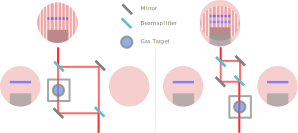
\includegraphics[width=1.0\columnwidth]{MachZehnder_Comparison.png}
\caption[Comparison of two Mach-Zehner interferometer geometries.]{Comparison of two Mach-Zehner (MZ) interferometer geometries. The laser beam (red) enters the sketch from the bottom and reaches the detector at the top. On its path it passes through a gas target (grey ring filled blue) in a vacuum chamber (grey box), where it images a plasma channel (blue-purple line). The pink circles indicate the respective beam properties on each arm. Left: Standard MZ setup. One propagates through the plasma, whereas the other beam bypasses it to act as reference. Both are fully overlapped to effect interference. Right: MZ setup used in the experiments at \textsc{Gemini}. A single beam passes through the plasma. The beam is then split up into two identical copies which are recombined with a spatial offset. Different regions of the beam act as reference and others as signal regions. Adapted from \cite{ColeThesis}.}
\label{Methods:Figs:MachZehnderComparison}
\end{figure}

In interferometry two beams are overlapped with a phase difference resulting in an interference pattern. One beam acts as the unperturbed reference, the second beam probes the perturbation of interest at the interaction point. Starting from the original interference pattern, the `fringes' will shift as the second beam collects phase shifts when propagating through the interaction region. In this context the phase shift, $\Delta \phi$, occurs due to density modulations in the plasma which are reflected in changes to the refractive index, $\eta$ \cite{Kaluza2019_ULTRAFAST,Hutchinson2002_PlasmaDiag}:
\begin{equation}
\Delta \phi(y,z) = \frac{2\pi}{\lambda} \int^\infty_{-\infty} (\eta(r,z) - 1) \mathrm{d}x,
\end{equation}
where the refractive index, $\eta$, is for underdense plasmas, $n_e \ll n_c$, approximated by $\eta \approx 1 - n_e/(2n_c)$.
\begin{equation}
\Delta \phi(y_0) = \frac{\pi}{n_c \lambda} \int^\infty_{-\infty} n_e (x, y_0) \mathrm{d}x = \frac{2 \pi}{n_c \lambda} \int^R_{y_0} \frac{n_e (r) r}{\sqrt{r^2 - y^2_0}}\mathrm{d}r,
\end{equation}
substituting $x = \sqrt{r^2 -y^2_0}$ and $\mathrm{d}r = r \mathrm{d}r/\sqrt{r^2 - y^2_0}$.
Assuming radial symmetry the plasma density $n_e (r)$ is then inferred using an Abel inversion \cite{FOURIER}:
\begin{equation}
n_e (r) = - \frac{n_c \lambda}{\pi^2}\int^R_r \frac{\mathrm{d}}{\mathrm{d}r}\Delta \phi(y) \frac{\mathrm{d}y}{\sqrt{y^2 - r^2}}
\end{equation}
More instructive details on this method can be found in \cite{ColeThesis}.
\vspace{\baselineskip}

In the experiments at \textsc{Gemini} described in this work a Mach-Zehnder interferometer was used. However, instead of splitting the beam before the interaction, the beam is only entering the Mach-Zehnder setup after the interaction, such that both copies are identical (see Figure \ref{Methods:Figs:MachZehnderComparison}). Since the plasma channel that is diagnosed only takes up a small fraction of the image, the remaining area of neutral gas can be used as reference. Similarly as in a Wollaston interferometer the two beams are offset relative to each other to overlap `active' with `passive' regions. As a result two copies of the plasma channel with inverted phase shifts can be seen.
An example of an interferometry measurement from an experiment performed at \textsc{Gemini} is shown in Figure \ref{Methods:Figs:Probe_Examples} (top).


\subsubsection{Experimental Implementation}

\begin{figure}[h]
\centering
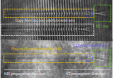
\includegraphics[width=0.75\columnwidth]{ProbeTA3.pdf}
\caption[Example of a shadowgraphy and an interferometry image taken on an experiment at \textsc{Gemini}.]{Example of an interferometry image (top) and a shadowgram (bottom) taken on an experiment at \textsc{Gemini} (see Chapter \ref{Chap:linICS}) on the same shot. Two laser pulses counterpropagate through a gas jet and form a plasma. One laser pulse is focused in an $f/40$ geometry (left to right), the other tightly by an $f/2$ off-axis parabola. The common features on both diagnostics are indicated in the same colour on both images.}
\label{Methods:Figs:Probe_Examples}
\end{figure}

In the LWFA experiments in this work the optical probe is split off the main wakefield driver beam by collecting the fraction of light that is transmitted through a highly reflective dielectric mirror. The transmitted light is telescoped down from $\sim 150\mm$, the beam diameter of the collimated main laser pulse, to about one inch using an $f/7$ off-axis parabola and a suitable lens. The final diameter is chosen based on the field of view required for the respective application. 

The collimated probe beam is then following a beam path of the same length as the main beam to ensure that both arrive at the interaction point simultaneously. 
The probe is send through the gas target at the interaction point and collects phase shifts encoding the density and its variation in the plasma. 
If the probe arrives before the main driver at the gas target, no plasma has been formed yet. If the probe arrives much later than the main beam the plasma channel it formed has expanded. 
As a result, the density measured is not representative of the conditions the driver beam experienced and in turn does not describe the wakefield dynamics correctly either. A motorised linear stage can be used to add or remove beam path dynamically (delay stage) to adjust the relative arrival time of the probe and the main beam. 

After the plasma the probe beam is attenuated by reflecting off glass wedges to prevent nonlinear effects when the laser pulse leaves the vacuum chamber through a glass window (B-integral). A set of lenses is used to image the plane of the gas target onto the prospective detector plane. On the way to the detector plane the probe pulse is split up by a beam splitter into two parts: one is directly incident on a CCD chip to act as shadowgraphy, the other pulse travels through a symmetric, compact Mach-Zehnder setup before also arriving at a CCD camera chip forming an interferometry diagnostic as outlined in the previous section.

Figure \ref{Methods:Figs:Probe_Examples} shows an example interferometry (top) and shadowgraphy (bottom) image, taken with an optical probe on the same shot. The data was taken on an experimental campaign at \textsc{Gemini} in 2019 (see Chapter \ref{Chap:linICS}). On the images an $f/40$ laser pulse is travelling through a helium gas jet and forms a plasma channel (gold). The centre of the channel is slightly darker and the edges form a bright line as discussed in the previous section. In the interferometry image, on the other hand, a shift of the interference pattern indicates the formation of a plasma channel. Due to the special setup of the Mach-Zehnder two copies of the same channel can be seen (white), where the only difference between the two is the inverted phase shift. On the right side the cone of a counterpropagating, tightly focused $f/2$ beam is visible (green). The particularly bright outline of the cone seen in the shadowgraphy indicates a large gradient in density. The distinct feature at the crossing of both pulses is potentially caused by an interaction between the optical probe pulse and the $f/2$ beam.


\iffalse
If one wants to capture smaller and more volatile features like the wake itself, a very short pulse duration ($\sim 10\,\mathrm{fs}$) for the probe pulse is required \cite{Siminos2016_FASTSHADOW} and very high resolution imaging \cite{Buck2011_BUBBLE,Savert2015_BUBBLE}. This represents a more direct measurement of the in-situ plasma conditions the laser and the wake experience (see also \cite{Kuschel2018_SELF}).
\fi

\section{Magnetic Energy Spectrometer}
\label{Chap:Methods:Sec:Espec}

The energy of electrons in wakefield experiments can be determined with a magnetic spectrometer, where electrons are dispersed in a magnetic field and then detected on a scintillating Lanex screen.
To analytically determine the deflection angle, $\theta$, in such a magnetic field, we will consider an external magnetic field restricted to a circle of radius $r_b$ embedded in an otherwise completely field-free region \cite{ManglesThesis}:
\begin{align}
\mathbf{B} &= B \mathbf{e_z} \, &r \leq r_b,\nonumber \\
&= \mathbf{0} &r > r_b
\end{align}
The angular deflection of a particle in this case can be solved analytically using the Larmor radius and simple geometry. This is visualised in Figure \ref{Methods:Figs:EspecAnalyticSketch} (left).
\begin{figure}
\centering
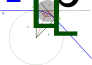
\includegraphics[width=0.49\columnwidth]{elecspec_2.pdf}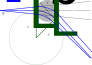
\includegraphics[width =0.49\columnwidth]{elecspec_3.pdf}
\caption[Visualisation of an electron deflected in a homogeneous magnetic field.]{Left: Visualisation of an electron deflected in a homogeneous circular magnetic field (grey) with radius $r_b$. The larger (empty) circle indicates the Larmor radius, determining the electron trajectory (blue) from the point of entry into the field (A) to its exit point (B) resulting in a total deflection $\theta$. Right: Similar visualisation as on the left but considering two electrons entering the same field at different angles and positions. }
\label{Methods:Figs:EspecAnalyticSketch}
\end{figure}
Since the sum of all angles in a triangle is $\pi$:
\begin{equation}
2 \alpha + \theta = \pi,
\end{equation}
where $\theta$ is the deflection angle and $\alpha$ the angle indicated in the sketch in Figure \ref{Methods:Figs:EspecAnalyticSketch} (left).
The angle $\alpha$ is geometrically related to the two radii:
\begin{equation}
\tan \alpha = \frac{r_L}{r_b}.
\end{equation}
By combining these results and expressing this in quantities relevant in an experiment we obtain
\begin{align}
\tan \frac{\theta}{2} &= \frac{r_b}{r_L},\nonumber\\
&= \frac{e B r_b}{p_\perp},
\end{align}
which indicates that at a fixed magnetic field strength, $B$, and field region, $r_b$, the deflection angle, $\theta$, is larger for a lower particle momentum, $p_\perp$, the to the magnetic field lines perpendicular momentum component. 
In a typical LWFA experiment $p_\perp$ will be dominated by the component in the laser propagation axis, i.e. if the propagation axis were $z$, $|\mathbf{p_\perp}| \approx p_z$. 
\vspace{\baselineskip}

In a realistic scenario the field regions are not perfectly homogeneous and field gradients have to be considered. The magnetic fields can be measured, for instance, using a Hall probe and the particle trajectories are determined with numerical methods.
To measure the magnetic dispersion as diagnostic a scintillating Lanex screen is positioned behind the magnet. By measuring the magnetic field strength of the magnet and the distances between the components, and by calculating the trajectories for a range of energies, each position on the screen can be linked to a specific electron energy. In this work a Matlab-based particle tracking code by Jonathan Wood (Imperial College) and another code by Matthew Streeter (Imperial College) were used (see Figure \ref{Methods:Figs:Espec_MattVis} for a visualisation from M. Streeter's code simulating the particle trajectories for the magnet configuration used in the photon-photon collider experiment outlined in Chapter \ref{Chap:BW}).

If all electrons enter the magnet at one defined position and angle each position on the detector screen is uniquely related to one electron energy. For a distribution of angles and positions each position on the screen can correspond to multiple energies (see Figure \ref{Methods:Figs:EspecAnalyticSketch}, right). 
In LWFA experiments variations in angle and position typically originate from two sources: 
first, the entire beam might be ejected from the accelerator at an angle relative to a reference axis that varies from shot-to-shot. 
This is referred to as \textit{beam pointing} and shifts the entire dispersed beam on the detection plane relative to the reference axis, i.e. leads to a systematic shift in the inferred energy if not considered.
Multiple detector screens or spatial references can be used to identify and correct for beam pointing \cite{Clayton2010_ION,Soloviev2011_TWOSCREEN,PoderThesis}.

Second, the beam has a finite divergence such that electrons entering the magnetic field have a distribution of angles, even at a fixed energy. 
As a result, one energy is not mapped onto a single point but a spot of finite size, i.e. the dispersion or energy axis and spatial components of the beam are mixed (instrument function).
\vspace{\baselineskip}

\begin{figure}
\centering
\includegraphics[width=1\columnwidth]{MagneticSpectrometer_Matt.png}
\caption[Visualisation of particle tracking in realistic fields.]{Example of particle tracking simulation using a code by M. Streeter (Imperial College). Electrons enter a three-piece magnet from the left side and are dispersed according to their energy (colour bar in electron energy). The perpendicular field magnet field component, $B_\perp$, is colour-coded, with black indicating zero and white $B_\perp = 1\,T$ (only valid within the black the rectangle, fields outside of it vanish). The vertical dashed line indicates the position of a measurement screen. }
\label{Methods:Figs:Espec_MattVis}
\end{figure}

The momentum component of the electron beam that is parallel to the magnetic field lines is unperturbed by the magnetic field as the magnetic Lorentz force vanishes for parallel vectors. If the size of the electron beam is very small at the end of the accelerator, measuring its width in the non-dispersed direction at the detector plane and the distance from the detector to the accelerator can be used to infer the magnitude of $p_\parallel$ relative to $p_\perp$, $p_\parallel/p_\perp$. This ratio is in the small-angle approximation equivalent to the angle to a reference axis $z$, with $z \parallel \mathbf{p_\perp}$, or applied to an entire beam the \textit{divergence}, $\theta$.
\vspace{\baselineskip}

\begin{figure}
\centering
\includegraphics[width=1.\columnwidth]{EspecMethods.png}
\caption[Example images of an electron spectrometer screen.]{Example images of an electron spectrometer screen. Left: Raw reference image of a Lanex spectrometer screen. The vertical axis is the dispersion axis, with the top part corresponding to less dispersion (higher energy), and the horizontal axis corresponds to divergence. Centre: Image on the left after applying a projective transform. Right: Example electron spectrum obtained using this setup and using particle tracking results to translate the spatial scale into an energy scale. This image was also background subtracted and cropped. The colour scale indicates charge per divergence and energy in arbitrary units (darker regions indicate more charge).}
\label{Methods:Fig:LanexExamples}
\end{figure}

In the experiments discussed in this thesis the detectors are scintillating Lanex screens (Kodak Standard or Biomax) imaged by cooled 16-bit CCD Andor Neo cameras. 
Since the imaging of the screens was non-normal but at an oblique angle to avoid placing the cameras into the path of the electrons, the spatial scale is not constant across the image. Spatial references on the image, here rulers attached to the frame holding the Lanex screen, can then be used to apply a projective transform that morphs the image onto a linear spatial scale \cite{ColeThesis, PoderThesis}. 
The linear spatial scale can then be translated into an energy axis in the dispersion direction, by applying the results from the particle tracking code described above, and into beam divergence in the non-dispersion direction (see Figure \ref{Methods:Fig:LanexExamples}, right).
This is shown in Figure \ref{Methods:Fig:LanexExamples} at an example image (from a Gemini campaign in 2015, experiment is described in more detail in Chapter \ref{Chap:RR15}). The panel on the left shows the raw reference image, with the rulers clearly visible on both sides and higher energies (less dispersion) at the top of the image. A projective transform has been applied to generate the image in the centre. Both sides are now straight and the spatial scale is slightly stretched in the upper part. On the right an example 2D electron spectrum is shown, obtained by replacing the spatial scale with an energy (vertical) and a divergence axis (horizontal) using the results from the tracking code, as well as subtracting background and cropping the image. The colour scale indicates charge per divergence and energy in arbitrary units.
The signal recorded from the Lanex screen can be related to the absolute number of electrons by cross calibrating with an imaging plate \cite{WoodThesis}.


\section{Gamma-ray Diagnostics}
\label{Methods:Sec:GammaDiags}

In the following diagnostics measuring the profile and spectrum of energetic radiation are introduced. Both detectors consist of a pixellated scintillator array imaged by a CCD camera. In one case the transverse profile of the radiation is measured, in the other case the gradual decay throughout several scintillating layers is used to infer the spectrum of the incident radiation.

At photon energies $> 1\MeV$ the quantum efficiency of CCD chips decreases significantly such that a direct measurement of the radiation using these becomes infeasible. Moreover, the production of particle showers can damage electronics in the radiation path. As a consequence, commercially available indirect detection X-ray cameras, e.g. Andor iKon, that directly couple a scintillating layer to a silicon-based readout chip are also not recommended to use in these energy ranges. By spatially separating the two components, i.e. placing the scintillator in the radiation path and the CCD sufficiently far away, this problem can be circumvented.

A scintillator placed into the path of the energetic radiation emits scintillation light when energy is deposited in the scintillator. 
A suitable imaging system collects the light and directs it onto the CCD detector. Commonly used scintillators emit light in a spectral bandwidth matched to the quantum efficiency of silicon-based detectors with a material-dependent characteristic emission spectrum. 
The light yield of the scintillator is at the energies relevant in this context proportional to the energy deposited in it \cite{Frlez2000_CsI}, with a material-dependent conversion efficiency from deposited energy to number of emitted photons. 
The light emission is isotropic in a $4\pi$ solid angle \cite{Birks2013_SCINTILLATOR}, which can lead to a spreading of the signal comparable to the thickness of the scintillator. 
This spreading can be reduced by either using a thin scintillator or by dividing the detection area into smaller scintillators such that light from one crystal can not enter another and vice versa. 
The result in the latter case is then a pixellated detector, where the spatial resolution is determined by the transverse width of the crystals such that deep (longitudinal) crystals can be used to increase the light yield without loss of spatial resolution. 
To increase the fraction of collected light the crystal faces are often polished and some sides are coated or covered with a reflective surface, so-called reflectors, such that the emitted scintillation can be directed. 

\subsection{Profile Screen}

Measuring the radiation profile is useful to measure, for instance, the pointing of the radiation cone and its divergence, or as indicator of the total radiation yield.
In the context of inverse Compton scattering or nonlinear relativistic Thomson scattering, where a relativistic electron beam is collided with an intense laser pulse, the elongation of the radiation profile in the laser polarisation direction has also been proposed as measurement of the laser intensity at the interaction \cite{HarShemesh2012_INTENSITY,Yan2017_ICS,Blackburn2019_ModelIndependentLaser}.

\begin{figure}
\centering
\includegraphics[height=0.3\columnwidth]{JenaProfile.jpg}\includegraphics[height=.3\columnwidth]{ScreenshotGEANT_JenaStack.png}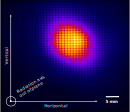
\includegraphics[height=0.3\columnwidth]{GammaProfileExample.pdf}
\caption[Scintillator profile screen, photograph, GEANT representation and measured gamma signal.]{Example of a scintillator stack (`Jena') used as profile screen in experiment. Photograph of the scintillator screen (left) along its GEANT representation (middle) and a false colour image of a gamma signal from linear inverse Compton scattering (right) measured with the stack in an experiment at \textsc{Gemini} in 2019 (Chapter \ref{Chap:linICS}).}
\label{Methods:Figs:GammaProfileExample}
\end{figure}

In the experiments described in this work a pixellated scintillating screen is placed into the path of the radiation, normal to the beam axis, and is then imaged by a sensitive EMCCD camera (Andor iXon) with a bandpass filter. 
An overview of the different arrays used in the experiments is given in Table \ref{Methods:Table:GammaProfileOverview}.
The imaging was in all cases done close to normal to the scintillator surface, either directly or by placing a mirror into the radiation path, to maximise the collection efficiency of the scintillation light which is directed due to the reflectors. This also reduces the required post-processing of the images to small rotations and background subtractions. In this setup the required spatial resolution of the imaging system is low as the intrinsic spatial resolution of the detector is given by the width of the scintillator voxels which are $\sim 1\mm$ or more.
The scintillating material that was used is caesium-iodide doped with thallium which has one of the highest light conversion efficiencies of available crystals releasing $\approx 5.4 \times 10^4$ optical photons at a central wavelength of $550\nm$ for each MeV energy deposited in the crystal \cite{StGobain_CsI}.

\begin{table}[h]
\centering
{\rowcolors{3}{white}{lightgray!50}
\begin{tabular}{|l|l|l|l|r|r|}
\hline
\multicolumn{6}{|c|}{\textbf{Overview of Scintillating Profile Screens}} \\ \hline \hline
\textbf{Name} & \textbf{Chapter} & \textbf{Crystals} & \textbf{Crystal Dim.} & \textbf{Front Plate} & \textbf{Divider}\\ \hline \hline
QUB & \ref{Chap:BW}, BW & $20 \times 20$ & $2 \times 2 \times 20$ mm & Al 10 mm & Al 0.1 mm\\
Jena & \ref{Chap:linICS}, linICS & $45 \times 45$ & $1 \times 1 \times 10$ mm & TiO2 0.5 mm & TiO2 0.2 mm\\
DESY & \ref{Chap:linICS}, linICS & $30 \times 30$ & $1.5 \times 1.5 \times 10$ mm & TiO2 0.5 mm & TiO2 0.2 mm\\
RAL & \ref{Chap:RR15}, RR & $47 \times 33$ & $5 \times 5 \times 50$ mm & None & Al 1 mm\\
\hline
\end{tabular}
}
\caption[Scintillator arrays used as profile screens in experiments.]{Overview of caesium-iodide arrays used as radiation profile screens in the context of this thesis. Columns from left to right: Name or `affiliation' of the screen, chapter related to an experiment using this particular profile screen, size of the array in number of crystal columns and rows, spatial dimensions of an individual crystal in the array, material and thickness of the front plate or coating on the front side facing the beam, divider material and thickness between crystals.}
\label{Methods:Table:GammaProfileOverview}
\end{table}


Figure \ref{Methods:Figs:GammaProfileExample} shows a photograph of one of the scintillating arrays used in this work (left, labelled `Jena' in Table \ref{Methods:Table:GammaProfileOverview}) along with a GEANT4 representation (centre) and a false-colour image of a detector response produced by a gamma-ray beam from inverse Compton scattering measured in the experiment at \textsc{Gemini} discussed in Chapter \ref{Chap:linICS}.
Each square corresponds to one crystal or voxel in the array.

\subsubsection{Energy dependent detector response}

\begin{figure}
\centering
\includegraphics[height=.3\columnwidth]{Edep_JenaStack.pdf}\includegraphics[height=.3\columnwidth]{Edep_Jena_1_100_MeV.png}
\caption[In GEANT4 simulated energy deposition in a gamma profile screen.]{In GEANT4 simulated energy deposition per photon in the `Jena' profile screen as a function of photon energy for 100 to 2000 keV (left) and 1 to 100 MeV photon energies (right).}
\label{Methods:Fig:EnergyDepGProfile}
\end{figure}

To determine the energy deposited in the scintillating crystals, one has to consider the scattering of the radiation, secondary particles and their energy deposition through various mechanisms. This complex interplay of different mechanisms is most conveniently modelled in a Monte-Carlo code such as GEANT4 since collective effects are not significant. Here a GEANT4 code was used based on work done by J. Cole and K. Poder (Imperial College). The simulation geometry includes the composition of the detector and the relevant materials in the beam path of the radiation as measured on the respective experiment. Individual photons within a range of energies are then launched towards the detector and the energy deposition is recorded as a function of the incident photon energies. For each photon energy $10^6$ photons are simulated to account for statistical fluctuations. In Figure \ref{Methods:Fig:EnergyDepGProfile} the energy deposited on average per incident photon in the `Jena' profile screen is shown as a function of the incident photon energy for an energy range of 100 to 2000 keV (left) and for 1 to 100 MeV. It is assumed that the light yield of the scintillator and the energy deposition are linearly related \cite{Frlez2000_CsI} and that there are no saturation effects to be considered in this scenario. 
With exception of a peak in energy deposition at just under 200 keV photon energy the energy deposited in the screen monotonically increases with photon energy. The distribution can in most parts approximated by two linear functions, one with a steep gradient up to a photon energy of 15 MeV and a second function with a lower gradient after this value.


\subsection{Spectrometer Array}
\label{Chap:Methods:subsec:GammaSpec}

\subsubsection{Experimental Setup}
A long array of scintillating crystals is placed in the beam path and its scintillation light is measured with a CCD. The spectrum of gamma radiation passing through the crystals is inferred by simulating the response of the array in GEANT4 \cite{GEANT4} and comparing it to the response measured in the experiment \cite{Behm2018_Gamma}.
A conceptual sketch of the experimental setup is shown in Figure \ref{Methods:Figs:SketchGammaSpec}: a beam of gamma rays (green) enters from the left side of the sketch, passes through a vacuum window (orange) into air, then traverses a lead collimator and enters the scintillator array. The crystals are indicated in yellow. The response of the detector is imaged by a camera (bottom right corner). 

\begin{figure}
\centering
\includegraphics[width=0.8\columnwidth]{GammaSpectrometerSketch.pdf}
\caption[Sketch of a gamma spectrometer setup in an experiment.]{Sketch of a gamma spectrometer setup in an experiment. The gamma rays (green) traverse from the left a vacuum window (orange) and then in air through a lead collimator onto an array of scintillators (yellow) housed in a casing. The stack is predominantly extended in the longitudinal direction (z) but can also resolve one transverse dimension (here y). A camera directly images the open side of the scintillator array.}
\label{Methods:Figs:SketchGammaSpec}
\end{figure}

The individual scintillators are caesium-iodide crystals doped with thallium, with the spatial dimensions $5 \times 5 \times 50\,\mathrm{mm}$. 
The long side of the crystals is oriented transversely to the propagation direction of the gamma rays ($z$), in the sketch shown in Figure \ref{Methods:Figs:SketchGammaSpec} this is the horizontal axis $x$ (see also Figure \ref{Methods:Figs:GammaSpectrometer_Axes}). This maximises the light yield as the response of the detector is integrated along this axis ($x$) but at cost of spatial resolution. The crystals are arranged in a two-dimensional grid of columns ($z$) and rows ($y$). Crystals along the longitudinal axis $z$ measure the decay of the radiation and can be used to infer the spectrum. The response in the $y$-axis encodes the vertical divergence of the radiation. 

The crystals are separated from each other by light-tight spacers such that each crystal is enclosed from all but one side, from which the scintillation light leaves the crystal. This crystal side faces in $x$ direction and the scintillation light is measured on a CCD. In all the experiments discussed in this thesis cooled 14-bit EMCCD cameras of type Andor iXon were used, which are very sensitive and allow for high gain but in turn also require efficient light shielding. The cameras were equipped with suitable objectives and bandpass filters that only transmit light in the bandwidth of the scintillation light at a wavelength of $546\pm10\nm$. A reflective casing for the crystals along with polishing and reflective coating of the crystals can increase the light output. 

The material and thickness of the dividers between the crystal columns determine how fast the incoming radiation decays which can be used to `tune' the response of the detector to the right spectral range. The separation and thickness of the crystals in the $y$-axis, on the other hand, determines the vertical spatial or, with respect to the radiation source, the angular resolution.
\vspace{\baselineskip}

Two different scintillator stack designs were used as gamma spectrometers in the experiments described in this thesis. An overview of the dimensions and the materials used in the arrays is provided in Table \ref{Methods:GSpec:Table} and photos of the stacks are shown in Figure \ref{Methods:Figs:CsI_Stacks}. Examples of raw images from both detectors are shown in Figure \ref{Methods:Figs:CsI_shotexemp}.



\begin{figure}
\centering
\includegraphics[height=0.3\columnwidth]{scintillator.jpg}\hspace{2em}%
\includegraphics[height=0.3\columnwidth]{DualAxis_assembly.JPG}
\caption[Photographs of scintillator arrays used in experiments.]{Photographs of scintillator arrays used in experiments. Left: `RAL' stack of $47 \times 33$ crystals. Right: Long dual-axis stack consisting of $10 \times 70$ crystals. More details can be found in Table \ref{Methods:GSpec:Table}}
\label{Methods:Figs:CsI_Stacks}
\end{figure}

\begin{figure}
\centering
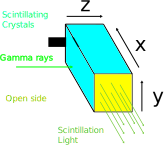
\includegraphics[height=0.3\columnwidth]{GammaSpecCrystals_2.pdf}\hspace{2em}%
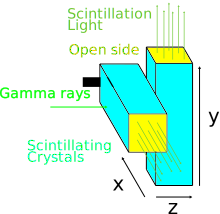
\includegraphics[height=0.3\columnwidth]{GammaSpecCrystals_3.pdf}
\caption[Sketch of crystal orientations in the spectrometer arrays relative to the incident gamma rays.]{Sketch of crystal orientations (cyan) in the spectrometer arrays relative to the incident gamma rays (green) for the RAL stack (left) and the alternating layers in the long dual-axis stack (right). The yellow faces indicate the open sides out of which the scintillation light (green) leaves the crystal.}
\label{Methods:Figs:GammaSpectrometer_Axes}
\end{figure}

In the experiment outlined in Chapter \ref{Chap:RR15} a $47 \times 33$ [longitudinal ($z$) $\times$ vertical ($y$)] array of crystals housed in an aluminium casing was used\footnote{Designed and built by Rob Clarke (CLF).} (see Figure \ref{Methods:Figs:CsI_Stacks}, left). The long side of the crystals was oriented along the horizontal direction ($x$) to maximise the light yield. The crystals were separated in $z$ and $y$ by 1-mm-thick light-tight aluminium spacers. On the sides ($x$) the array is held together by 1-mm-thick aluminium plates. One plate is solid, on the other side 4 mm diameter holes over the crystal faces allow the scintillation light to escape. The aluminium spacers and the solid plate reflect the light and direct the photons towards the only open side. The front and back side of the stack ($z$) are fortified with $9\,\mathrm{mm}$ thick steel plates.

The experiment described in Chapter \ref{Chap:BW} used the same scintillator array as above for the setup described in Chapter \ref{Chap:RR15}, but the thick steel front plate is replaced by a 1-mm sheet of plastic (PTFE) to reduce the attenuation of the incident radiation. In this setup a scintillating profile screen is placed in front of the spectrometer array (see previous section). The additional material of the profile screen roughly compensates the effect of the thinner front plate and matches the response of the detector to its previous configuration. 
\vspace{\baselineskip}


\begin{figure}
\centering
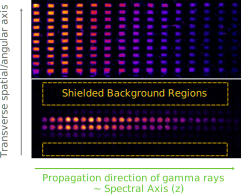
\includegraphics[width=.6\columnwidth]{GammaSpecExamples.pdf}
\caption[Examples of raw response recorded on scintillator arrays.]{Examples of raw response recorded on scintillator arrays in false colour, where black indicates low and orange a high signal. The radiation propagates into the stack from left to right, such that radiation of higher energy penetrate deeper into the stack. The vertical axis encodes spatial/angular information. Top: Top view of the first 15 crystal columns of the dual-axis stack. The response was measured at \textsc{Gemini} in 2019. Each square is an individual crystal, where the different dimensions are due to a large variation in the size of the transverse spacers that were used in the assembly. Top: Response of the `RAL' spectrometer stack to gamma radiation from inverse Compton scattering measured at \textsc{Gemini} in late 2015 (see Chapter \ref{Chap:RR15}). The stack was housed in a lead enclosure with a circular aperture (lead collimator) such that the signal area is restricted to the centre. The shielded regions can be used as background measurement. The crystals in this array have also rectangular faces but the casing holding the crystals in place has round apertures.}
\label{Methods:Figs:CsI_shotexemp}
\end{figure}


In the campaign described in Chapter \ref{Chap:linICS}, a longer array of $10 \times 70$ [transverse ($x,y$) $\times$ longitudinal ($z$)] crystals was fielded\footnote{Proposed by Stuart Mangles (IC), designed and built by D. Treverrow (CLF) and C. Baird (CLF).} (see Figure \ref{Methods:Figs:CsI_Stacks}, right). Since the gamma beam produced in these experiments is highly-directional, the signal measured in previous experiments on the array described above was concentrated on a few central rows with a large number of crystals being left unused. In this design the transverse dimension is reduced in favour of an extension in the $z$ axis that is spectrally relevant. In addition, lighter spacing materials are used to slow down the decay and stretch out the signal over more crystal columns ($z$).

The crystals rows ($x,y$) are spaced by black polyethylene dividers and the columns by $0.5\,\mathrm{mm}$ sheets of black nylon. The small faces of the crystals that are not imaged are covered with reflective aluminium foil. The front plate of the stack is a $2\,\mathrm{mm}$ thick aluminium plate. The entire stack is held together by an aluminium skeleton, with the 4 long sides being covered by transparent PTFE plastic sheets. 
The positioning and visibility of the crystals is less regular than in the other stack since this array was assembled from hundreds of individual components which were partly not matching the requested dimensions, requiring manual (and hence not completely repeatable) corrections. In addition, the light shielding of the extremal rows (see Figure \ref{Methods:Figs:CsI_shotexemp} (top)) appears to require improvement as well.

Another new feature of this array is the alternating orientation of the crystals (see Figure \ref{Methods:Figs:GammaSpectrometer_Axes}, right): the long side of the crystals is now in every other column rotated from the $x$-axis (horizontal) by $90$ degrees to align with the $y$-axis (vertical). Each odd and even layer now integrates the response of the detector in a different transverse dimension. The preserved non-integrated spatial component then also alternates with each subsequent column. This is discussed in more detail at the end of this section.

In the setup outlined in Chapter \ref{Chap:linICS} the top of the detector ($y$) was imaged directly and a long rectangular mirror was placed at 45 degrees next to the other side, reflecting the scintillating light from even and odd layers onto the same CCD chip to use the area of the rectangular CCD chip most efficiently. Due to the length of the stack ($z$) two cameras were used, one for the front section and one for the back. 


\begin{table}
\centering
{\rowcolors{3}{white}{lightgray!50}
\begin{tabular}{|l|l|l|r|r|}
\hline
\multicolumn{5}{|c|}{\textbf{Overview of Spectrometer Arrays}} \\ \hline \hline
\textbf{Name} & \textbf{Chapter} & \textbf{Crystals} &  \textbf{Front Plate} & \textbf{Divider}\\ \hline \hline
RAL & \ref{Chap:RR15}, RR & $47 \times 33$ & Steel 9 mm & Al 1 mm\\
RAL & \ref{Chap:BW}, BW & $47 \times 33$ & PTFE 1 mm & Al 1 mm\\
Dual & \ref{Chap:linICS}, linICS & $10 \times 70$ & Al 2 mm & Nylon 0.5 mm\\
\hline
\end{tabular}
}
\caption[Scintillator arrays used as spectrometers in experiments.]{Overview of scintillator arrays used in the experiments discussed in this thesis and their properties, namely the array size, divider and front plate material. The material of all crystals that were used is caesium-iodide doped with thallium and have the spatial dimensions $5 \times 5 \times 50$ mm.}
\label{Methods:GSpec:Table}
\end{table}

\subsubsection{GEANT Simulation Setup}

The attenuation and energy deposition of the radiation is simulated using the Monte Carlo code GEANT4 \cite{GEANT4} as the impact of secondary radiation and particles as well as 3D effects such as side-scattering become important.
The specific GEANT4 code used in this work builds on previous work by K. Poder and J. Cole (Imperial College).


\begin{figure}
\centering
\includegraphics[height=0.25\columnwidth]{Screenshot_GEANT4_RALStack_BW.png}\includegraphics[height=0.25\columnwidth]{ScreenshotGEANT_DualAxisStack.png}
\caption[GEANT representations of the two scintillator arrays used in the experiments]{GEANT representations of the two scintillator arrays used in the experiments without their outer casing. The cyan blocks indicate the caesium-idodide crystals and the energy deposited in those volumes is recorded as detector response. Divider materials, front- and end plates are indicated in white. Photos of the stacks are shown in Figure \ref{Methods:Figs:CsI_Stacks}.}
\label{Methods:GSpec:GEANT4screenshots}
\end{figure}

Typically $10^{6}$ individual photons or $10^5$ electrons are simulated, assuming collective or multi-photon/-particle processes are negligible, such that individual photon responses can be combined cumulatively. The specific experiment geometries are reconstructed in GEANT4 including the detector geometry and materials in the pathway as well as distances measured in the experiment. The GEANT4 representations of the two spectrometer designs are shown in Figure \ref{Methods:GSpec:GEANT4screenshots}. The electrons and gamma rays are emitted from a point source and low divergence, close to an idealised pencil beam. 
The code measures the energy deposition in the scintillator material, but does not model the physics of the scintillation process itself or the light transport. It is assumed that the energy deposited within the scintillator crystals is linearly related to the light yield of the scintillator, i.e. the number of fluorescence photons emitted, independent of the process of energy deposition \cite{Frlez2000_CsI}.


\subsubsection{Image processing and background subtraction}

The response of the scintillator array is recorded as an image on a CCD and the images require processing before analysing them.
The specific steps vary from setup to setup depending on the imaging system. The open side of the crystals (see Figure \ref{Methods:Figs:GammaSpectrometer_Axes}) were imaged close-to-normal to collect a large fraction of the scintillation light, which also removed the necessity of morphing the image as required for the magnetic spectrometer screen (see Section \ref{Chap:Methods:Sec:Espec}).

\begin{figure}
\centering
\includegraphics[trim={4.8cm 0 5cm 0}, clip, width=1.\columnwidth]{GSpec_Example_Betamax_BGSub_Top.png}
\caption[Images of the dual-axis spectrometer stack before and after background subtraction.]{Images of the dual-axis spectrometer stack before (left) and after background subtraction (right), excluding treatment of bremsstrahlung. The colour scale is matched to the lowest and highest pixel value on the respective image.}
\label{Methods:Figs:GSpec:BGsub}
\end{figure}

The images contain background noise from different sources that have to be removed. The background can roughly be divided into continuous off-shot background and on-shot noise. The off-shot noise includes the intrinsic `dark noise' on the camera chip and counts related to ambient light.
This background can be characterised by taking a series of images at dark conditions which are then subtracted from on-shot data.

In high-intensity laser-plasma interactions energetic radiation and particles are produced, which can directly hit CCD chips resulting in `hard hits' or `hot pixels'. In addition the scattered laser light and bremsstrahlung might produce a signal on the detectors. 
Scattered laser light can be mitigated by putting light shielding in place and adding bandpass filters to the imaging system with a transmission that is matched to the bandwidth of the scintillation light. Hard hits, single pixels with high or saturation value, can be removed by applying a median filter which will also result in some blurring of the image. The treatment of the bremsstrahlung background is more complicated and will be discussed later.

In the experiment outlined in Chapter \ref{Chap:RR15} the radiation signal is constrained to a narrow, central part of the image due to the lead collimator and the remaining image can be used as on-shot reference to account for off-shot noise and on-shot noise from stray light (see Figure \ref{Methods:Figs:CsI_shotexemp}).
In Chapters \ref{Chap:linICS} and \ref{Chap:BW} the signal occupies large parts of the image and the regions in between the crystals are used instead to estimate the background. An explicit example of a background subtraction is shown in Figure \ref{Methods:Figs:GSpec:BGsub}. On the left an image of the raw detector response to hard betatron radiation. The colour scale indicates the number of pixel counts and is scaled to the minimum and maximum values on the image. Due to efficient shielding the camera is not affected much by `hard hits', but some of the crystals (squares) are barely visible. On the right the image after the background subtraction is shown, where the colour scale is again matched to its minimum and maximum values. The contrast has improved significantly, such that each crystal is clearly visible.
\vspace{\baselineskip}

\begin{figure}
\centering
%\includegraphics[height=0.25\columnwidth]{CsI_CrystalExtrExample.png}\includegraphics[height=0.25\columnwidth]{CsI_CrystalExtrPixExample.png}
%\includegraphics[width=1.0\columnwidth]{DualAxisCrystalExtrExample.png}
%\includegraphics[height=0.25\columnwidth]{CsI_CrystalExtrExample_Int.png}\includegraphics[height=0.25\columnwidth]{CsI_CrystalExtrPixExample_Int.png}
\includegraphics[trim={4.8cm 0 5cm 0}, clip, width=0.5\columnwidth]{CrystalExtract_Example_Full.png}\includegraphics[trim={4.8cm 0 5cm 0}, clip, width=0.5\columnwidth]{CrystalExtract_Example_Pixelated.png}
\caption[Response of a scintillator stack as measured by the detector and its pixellated response.]{Response produced by an LWFA bremsstrahlung source measured using the dual-axis spectrometer stack. The radiation enters the stack from the left side and propagates to the right. Left: Image of the scintillator stack after background subtraction. The black rectangles indicate the regions of interest where the crystals are located. The dark regions in between the crystals are occupied by spacers. Right: Corresponding pixellated response retrieved from the image on the left by integrating over the regions indicated by the rectangles.}
\label{Methods:Figs:GSpec:Pixellated_Response}
\end{figure}


Even with efficient filling of the field of view, the crystals emitting the scintillation light only occupy a fraction of the total image.
To further reduce the impact of noise and to focus on the signal-relevant parts of the image, we select the regions of the individual crystals (see Figure \ref{Methods:Figs:GSpec:Pixellated_Response}) and extract the content of the crystals. The result is a pixellated response of the detector, only using its active parts.
The shape of the decay in the longitudinal direction is characteristic of the spectral content, whereas the transverse dimension indicates the angular divergence. The transverse width of the crystal and spacers determine the transverse spatial resolution.


\subsubsection{On-shot bremsstrahlung background and shielding}

In the experiment setups described in this thesis, electrons are accelerated and dispersed in a magnetic spectrometer. While traversing the chamber and also when leaving it, the electrons interact with a range of solid materials, resulting in scattering, generation of secondary particles and showers of bremsstrahlung being produced. This is another source of on-shot noise. Since the radiation from this process is highly energetic, a lot of energy is potentially deposited in the scintillator crystals dominating the detector response.
\vspace{\baselineskip}

Consequently, it is important to reduce the amount of noise reaching the detector by identifying the main source and shielding the direct line of sight to the detector efficiently. 
In the setup described in Chapter \ref{Chap:linICS}, the electrons were dispersed sideways and the detector was shielded with lead on both of its sides.
In the campaign reported of in Chapter \ref{Chap:RR15}, the electrons were dispersed upwards. The main source of noise is the roof of the vacuum chamber and the ceiling of the target area. After measuring the shower of radiation from above on the detectors, the top of the detector was shielded with lead which reduced the noise level. A lead collimator was also used to limit the acceptance angle for radiation coming from upstream (see Figures \ref{Methods:Figs:SketchGammaSpec} and \ref{Methods:Figs:CsI_shotexemp}).
For the measurements in Chapter \ref{Chap:BW}, the electrons were primarily dispersed downwards into the thick breadboard of the vacuum chamber, the chamber itself and the floor of the target area. Two lead walls with narrow apertures and a large aperture 60-cm-long magnet were blocking the direct line of sight downstream to the detector (see Figure \ref{BW:fig:exp_sketch}). In some instances the primary magnet was removed from the setup and the second magnet was used to characterise the electron beam by dispersing it horizontally. To account for this scenario the sides of the detector were shielded with lead as well.
\vspace{\baselineskip}

Since the primary noise source is off-axis, efficient shielding of the direct line of sight reduces the measured signal significantly. Most of the remaining radiation is then entering the detector on the same path as any radiation signal we would want to characterise. 
As a result, it is impossible to shield this component without infringing on the signal itself, but the response of the detector can be used to characterise the background. On shots with the background and the signal present, on the other hand, the detector response is then the combined response to both, and depending on their relative yields the spectral retrieval of the signal might be affected.

In the results presented in this thesis gamma rays produced by three methods are characterised.
Each generation method requires a slightly different approach to deal with the bremsstrahlung background which are briefly discussed here.
\begin{enumerate}
\item Linear inverse Compton scattering (Chapter \ref{Chap:linICS}): The background was characterised by a series of null shots, i.e no scattering laser, but the full electron beam. The spectral shape of the background was found to be stable and its total yield proportional to the total energy in the electron beam, $Q \langle \gamma^2 \rangle$, where $Q$ is the total beam charge and $\gamma$ is the electron Lorentz factor. As linear inverse Compton scattering does not affect the energy of the electron beam this allows the measured electron spectrum on full shots to be used to estimate the bremsstrahlung background on each shot.
\item Non-linear inverse Compton scattering (Chapter \ref{Chap:RR15}): The background was characterised on a series of null shots and was also found to be proportional to $Q \langle \gamma^2 \rangle$. Although the energy spectrum is affected by collision with the laser on full shots, the bremsstrahlung sources are likely to be from interaction of electrons with material downstream from the collision point. This means it is reasonable to assume that the background on full shots is determined by the post-collision $Q \langle \gamma^2 \rangle$.
\item Bremsstrahlung (Chapter \ref{Chap:BW}): The background, characterised on shots without the converter in place, was much lower than the signal measured on shots with the converter. The background therefore has a negligible affect on the measured spectrum when the converter was used.
\end{enumerate}

\subsubsection{Detector Calibration using Bremsstrahlung}

The conversion efficiency of the scintillator varies from crystal to crystal. This might be due to differences in quality of the crystal, radiation damage or age.
The light emitted from the stack might also vary due to small changes in the dividers, polishing, or positioning of the crystal.
Finally, the relative measured signal is also affected by a varying viewing angle and collection efficiency across the image. 

To be able to compare the simulated response and the experimentally measured response, we have to match both through a suitable calibration.
In order to correct all the different factors using one calibration, we have to use a well understood comparable test signal in the right energy range that we can simulate and measure in an experiment. By comparing the simulated and measured response we then obtain a correction factor for each crystal.

A well understood mechanism with a spectrum covering a wide range is bremsstrahlung from relativistic electrons interacting with solid foils. The overall spectral shape is also only weakly dependent on the spectral shape of the used electron spectrum. Using a relativistic electron beam we can produce a directed bremsstrahlung source.

In the experiments described in this thesis electrons are accelerated via LWFA and characterised using a magnetic spectrometer.
A foil of known material and thickness is then inserted into the path of the undispersed electrons to produce a directed beam of bremsstrahlung generating a detector response. If we know the properties of the electron beam and the converter material (material, thickness) we can simulate the expected bremsstrahlung spectrum and the corresponding detector response in GEANT4 to compare with the experimentally measured response. Throughout this work various background methods were used, which are summarised in Table \ref{Methods:Table:BremsstrahlungCalibrationConverters}.

\begin{figure}
\centering
\includegraphics[width=.5\columnwidth]{Example_BremsGEANT_ElecInput.png}\includegraphics[width=.5\columnwidth]{Example_GSpecGEANT_GammaSpec.png}
\caption[Example of simulated bremsstrahlung spectrum using electron spectra measured in experiment.]{Left: Two examples of electron spectra measured in an experiment that are used as input for GEANT4 bremsstrahlung simulation. Right: Corresponding simulated bremsstrahlung spectrum produced using 1 mm of bismuth as converter material. The spectrum is normalised by the number of electrons in the simulation.}
\label{Methods:Figs:GEANTGamma_Elec}
\end{figure}




\begin{table}[h]
\centering
{\rowcolors{3}{white}{lightgray!50}
\begin{tabular}{|l|l|r|r|}
\hline
\multicolumn{4}{|c|}{\textbf{Calibration Targets and Methods}} \\ \hline \hline
\textbf{Chapter} & \textbf{Converter} & \textbf{On-/Off-Shot} & \textbf{Collimation}\\ \hline \hline
\ref{Chap:linICS} & 1.6 mm PTFE & on-shot & Narrow\\
\ref{Chap:RR15} & 9 mm Pb & off-shot, statistical & Wide\\
\ref{Chap:BW} & 4 mm W & off-shot, statistical & Wide\\
\hline
\end{tabular}
}
\caption[Overview of bremsstrahlung converter targets used for the calibration.]{Overview of bremsstrahlung converter targets used for the calibration. The PTFE converter enables measuring the electron beam on-shot, whereas the other targets lead to strong scattering and the electron beam is characterised statistically.}
\label{Methods:Table:BremsstrahlungCalibrationConverters}
\end{table}



In Figure \ref{Methods:Figs:GSpecBremsResponse_ExpAndSim} an example of an experimentally measured and a simulation result for one detector row is presented. The simulated response is very smooth in comparison to the measured response, where the peaks in the experimental data are results of the varying light efficiency of the crystals (intrinsic to the crystals and the setup). 
By dividing the simulated response by the experimentally measured response we obtain one correction factor, $c_{corr} (i, j)$, for each crystal in an array of $(i\, \times\,j)$ crystals:
\begin{align}
c_{corr}(i,j) &= \frac{R_{sim}(i,j)}{R_{exp}(i,j)},\\ \nonumber
c_{corr} &= R_{sim} \, \oslash \, R_{exp}.
\label{Methods:Eqns:GSpec_CorrFactor}
\end{align}

\begin{figure}
\centering
%\includegraphics[width=.5\columnwidth]{Example_BremsGEANT_ElecInput.png}\includegraphics[width=.5\columnwidth]{Example_GSpecGEANT_GammaSpec.png}
\includegraphics[width=.5\columnwidth]{Example_GSpec_ExpSim.png}\includegraphics[width=.5\columnwidth]{Example_GSpecGEANT_Corr.png}
\caption[Determining a correction factor to match the in GEANT simulated and measured detector response.]{Left: Measured experimental response of the detector for bremsstrahlung (blue) and the corresponding in GEANT simulated response curve (orange). Both curves are normalised to their maximum value. Right: Correction factor for the crystal rows obtained by dividing the simulated by the experimentally measured detector response (Eqn. \eqref{Methods:Eqns:GSpec_CorrFactor}).}
\label{Methods:Figs:GSpecBremsResponse_ExpAndSim}
\end{figure}

This correction factor now accounts for deviations in the efficiency independently of its origin (e.g. imaging setup, intrinsic crystal efficiency).
To reduce the experimental error this can also be averaged over several shots, but experimental data has shown that bremsstrahlung is a very reliable and reproducible source \cite{Behm2018_Gamma}. However, if the detector is moved or the imaging is being changed, the procedure has to be repeated.
The `corrected' response, $R_{corr}$, is then being obtained by multiplying the experimental response of crystal $(i,j)$ in the array, $R_{exp}(i,j)$, by the corresponding correction factor $c_{corr}(i,j)$:
\begin{align}
R_{corr}(i,j) &= R_{exp}(i,j) \,\cdot \,c_{corr} (i,j), \\ \nonumber
 R_{corr} &= R_{exp} \, \circ \, c_{corr}.
\end{align}

\subsubsection{Detector response for gamma-ray spectra}

Since we obtained the background-subtracted detector response and corrected the response for experimental deviations from an idealised detector, we can proceed to characterise the energy-dependent response and infer a gamma spectrum from experimental data.
As we will use the same setup and detector to characterise different types of radiation with different spectral shapes, we will use a generalised technique that will flexibly work in different scenarios.

First, we run GEANT simulations similarly as before for the bremsstrahlung calibration, but now for mono-energetic gamma rays covering the energy range of interest. The characteristic shape of the energy deposition in the longitudinal crystal rows and its variation with photon energy can be seen in Figure \ref{Methods:Figs:GSpec_GEANT} (left) for up to 500 MeV gamma rays. The simulated energy deposition ramps up to a peak before decaying, with the peak moving further into the stack with increasing photon energies. This is a result of the showers of secondary radiation and particles the energetic photons produce when interacting with the material of the stack. The position of this peak is hence an indicator of the length of this cascade and the energy of the radiation that is incident on the stack. 

Figure \ref{Methods:Figs:GSpec_GEANT} (right) shows the crystal which records the highest energy deposition as a function of photon
energy. The different curves show how this changes in different detector geometries. By adding more material before the stack or using dense high-Z materials the highest energy deposition occurs earlier and, inversely, using plastic instead of metal can be used to move the peak further into the stack. This means that the choice of materials can be used to compress or stretch parts of the signal over more or fewer crystals.
\vspace{\baselineskip}
\begin{figure}
\centering
\includegraphics[width=.5\columnwidth]{EdepGEANTStack.png}\includegraphics[width=.5\columnwidth]{EdepMax_Cases.pdf}
\caption[Simulated detector response to mono-energetic photons and different detector setups.]{Left: Detector response to mono-energetic gamma-rays simulated in GEANT4, using a setup as in Chapter \ref{Chap:BW}. The energy deposited per photon from energies 10 to 500 MeV is shown as function of the longitudinal crystal row. The photon energy is encoded in the colour axis from low (black) to high (white). The energy deposition per crystal rises to a maximum and then decays further into the stack. Right: Crystal recording the highest energy deposition as a function of photon energy for different detector geometries: `RAL' stack with steel front plate (blue), additionally a gamma profile screen (`QUB'), `RAL' stack with front plate replaced by PTFE and profile screen, dual-axis detector with profile screen (see also Tables \ref{Methods:Table:GammaProfileOverview} and \ref{Methods:GSpec:Table}). In general, the peak of the response increases with increasing photon energies, where fluctuations are probably caused by statistical fluctuations in the simulated data and would vanish for larger simulation sets.}
\label{Methods:Figs:GSpec_GEANT}
\end{figure}

We now simulated the energy deposition for a range of incoming photon energies in terms of energy deposition for crystals in longitudinal direction for a given photon energy. We assume this is linearly converted into light output  \cite{Frlez2000_CsI} and that the experimental measurement has been corrected as described previously. For each photon energy $E_i$ we obtain an array of deposited energies $\mathbf{R_i}$ in the longitudinal crystal columns $C_1$ to $C_n$ 
\begin{eqnarray}
\mathbf{R_i} = & \bordermatrix{\text{}&C_1&C_2&\ldots &C_n\cr
                E_i&R_{i1} &  R_{i2}  & \ldots & R_{in}} 
\end{eqnarray}
where $R_{ij}$ is the energy deposited in crystal $j$ by a photon of energy $E_i$.
We can expand this to a matrix of energies in one direction and energy deposition in a particular longitudinal row. To reduce the number of simulations we require, we can interpolate the detector response on a finer grid of photon energies, filling in energies between the simulated photon energies. The energy deposition is normalised such that it represents the energy deposited by one single photon of the respective energy. If we do this for $m$ different photon energies for a longitudinal array of $n$ crystals, we obtain an $m \times n$-sized matrix $\mathbf{R}$:
\begin{eqnarray}
\mathbf{R} = & \bordermatrix{\text{}&C_1&C_2&\ldots &C_n\cr
                E_1&R_{11} &  R_{12}  & \ldots & R_{1n}\cr
                E_2& R_{21}  &  R_{22} & \ldots & R_{2n}\cr
                \vdots & \vdots & \vdots & \ddots & \vdots\cr
                E_m & R_{m1}  &   R_{m2}       &\ldots & R_{mn}} 
\end{eqnarray}
An entry $R_{ij}$ is then the energy a photon of energy $E_i$ deposits in the longitudinal crystal row $j$.
Each row is the individual contribution of one photon at a defined energy and by summing several rows and weighting them according to a spectrum, we determine the combined response of the detector.
This can also be expressed more generally in terms of a matrix multiplication.
Define a vector $\mathbf{N}$ of length $m$. Each entry is the number of photons or relative weight $N_i$ of energy $E_i$ in an arbitrary gamma spectrum.
\begin{eqnarray}
\mathbf{N} = & \bordermatrix{\text{}&E_1&E_2&\ldots &E_m\cr
               &N_{1} &  N_{2}  & \ldots & N_{m}} 
\end{eqnarray}
Multiplying the vector $\mathbf{N}$ containing the spectral information of the gamma spectrum with the response matrix $\mathbf{R}$ is equivalent to calculating the combined response or signal $\mathbf{S}$ of all photons in the spectrum defined by $\mathbf{N}$. $\mathbf{S}$ is then a vector of length $n$, the number of longitudinal crystals.
\begin{eqnarray}
\mathbf{S}=\mathbf{N} \mathbf{R} =  \bordermatrix{\text{}&E_1&\ldots &E_m\cr
               &N_{1}  & \ldots & N_{m}} & \bordermatrix{\text{}&C_1&\ldots &C_n\cr
                &R_{11}  & \ldots & R_{1n}\cr
               & R_{21}   & \ldots & R_{2n}\cr
               & \vdots  & \ddots & \vdots\cr
                 & R_{m1}       &\ldots & R_{mn}} =\bordermatrix{\text{}&C_1&\ldots &C_n\cr
               &S_{1}   & \ldots & S_{n}} 
\end{eqnarray}
Each entry of $\mathbf{S}$ is then
\begin{equation}
S_i = \sum_{j=1}^{m} R_{ij} N_j,
\end{equation}
i.e. the sum of responses for the longitudinal crystal row $i$ for all photon energies weighted by the spectrum $\mathbf{N}$.
Provided we have access to a sufficiently populated matrix that spans a wide energy range, we can calculate the response of the detector associated to any arbitrary spectral shape.

Since this is a matrix operation, the experimental response of the detector can in theory be inverted to obtain the input spectrum. Unfortunately, noise and the low sensitivity of the detector response to smaller changes in the spectral shape make an inversion an unsuitable technique. Instead we assume a parametrised spectral shape, calculate the response for a range of parameters and find the best fit to the experimentally measured response, for instance using a least-square fit. 
Other work has shown that the gamma spectrum can be retrieved without assumption of the spectral shape if a second independent measurement is performed, for instance using a Compton or pair spectrometer \cite{Lisi2018_Gamma}.

\subsubsection{Resolving spatial features}

Due to the comparatively large crystals used in the spectrometer arrays the spatial resolution of both detectors is poor compared to the profile screens introduced in the previous section. In addition, the long crystals that are used to increase the light yield also destroy one of two transverse spatial components of the radiation.
In the dual-axis stack, however, the orientation of the crystals is alternated and, as a result, the spatial dimension that is resolved (or destroyed) alternates as well (see Figure \ref{Methods:Figs:GammaSpectrometer_Axes}). 

\begin{figure}
\centering
\includegraphics[width=0.9\columnwidth]{GammaSpec_Views.pdf}
\caption[Sketch of a combined setup of a gamma profile screen and a dual-axis spectrometer.]{Sketch of a combined setup of a gamma profile screen (green) and a dual-axis spectrometer (gold) along with example data from a bremsstrahlung source at \textsc{Gemini}. For the dual-axis spectrometer the two views enabled by the alternating crystal layers are indicated in purple (vertically integrated) and blue (horizontally integrated), with the associated experimental data marked in the same colours.}
\label{Methods:Figs:Dual-axis_Profile_Combo}
\end{figure}
Figure \ref{Methods:Figs:Dual-axis_Profile_Combo} shows a sketch of a combined setup using a profile screen (green) and the dual-axis spectrometer (gold) along with example on-shot data for the diagnostics from bremsstrahlung that was taken on an experiment at \textsc{Gemini} (see Chapter \ref{Chap:linICS}).
The experimental data is shown in a larger format in Figure \ref{Methods:Figs:Spatial} (top). 
The gamma beam from bremsstrahlung is narrow and symmetric such that it produces a small circle on the gamma profile screen (left) and is concentrated only on one or two crystal rows in the vertically integrated (centre) and horizontally integrated response (right). 
Assuming that the gamma beam is confined to an expanding cone centred around an axis parallel or at a small angle to the nominal laser axis, the centroid and the bright rows visible on the two projections can be used to confirm the relative position of the two detectors within their spatial/angular resolution. At the specific example of the data provided in Figure \ref{Methods:Figs:Spatial} (top): the positions of crystal row $8$ on the vertically integrated view and row $4$ on the horizontally integrated response correspond to the area around pixel $(x,y) \sim (180,120)$ on the gamma profile screen. This can be confirmed further by observing how the signal shifts on all three views relative to each other as a result of beam pointing.

The spatial resolution is determined by the size of the crystals and their spacing, which is $5+1\mm$ for the RAL stack and $5+0.5\mm$ for the dual-axis stack (see Table \ref{Methods:GSpec:Table}). The RAL stack is very wide and covers a height of $198\mm$, whereas the dual-axis stack covers $55\mm$. At $3\,\mathrm{m}$ distance from the source this then corresponds to an angular resolution of $2\mrad$ and $1.83\mrad$ at a field of view of $66\mrad$ and $18.33\mrad$, respectively. 


\begin{figure}
\centering
\includegraphics[trim={2.0cm 0 3cm 0}, clip, height=0.23\columnwidth]{GammaProfile_Brems_example.png}\includegraphics[trim={4.8cm 0 5cm 0}, clip, height=0.23\columnwidth]{GSpec_Example_Spatial_Brems_Top.png}\includegraphics[trim={4.8cm 0 5cm 0}, clip, height=0.23\columnwidth]{GSpec_Example_Spatial_Brems_Side.png}

\includegraphics[trim={2.0cm 0 3cm 0}, clip, height=0.23\columnwidth]{GammaProfile_Betamax_example.png}\includegraphics[trim={4.8cm 0 5cm 0}, clip, height=0.23\columnwidth]{GSpec_Example_Spatial_Betamax_Top.png}\includegraphics[trim={4.8cm 0 5cm 0}, clip, height=0.23\columnwidth]{GSpec_Example_Spatial_Betamax_Side.png}
\caption[Dual-axis detector response to symmetric and asymmetric gamma sources.]{Gamma signal measured in experiment with a gamma profile screen (left) and the corresponding pixellated detector response of the dual-axis scintillator stack. Two views of the array, integrated vertically (middle) and horizontally (right), are shown for a symmetric bremsstrahlung source (top) and elongated betatron radiation (bottom). The transverse crystal (y-axis) indicates pointing and the spatial extent of the source. The symmetric source produces a comparable response in views. The betatron source produces a narrow response in the horizontally integrated axis as most energy is deposited in a single crystal, whereas its response is spread widely in the other axis.}
\label{Methods:Figs:Spatial}
\end{figure}

In Figure \ref{Methods:Figs:Spatial} (bottom), on the other hand, the response of an asymmetric gamma beam from hard betatron radiation is shown. On the profile screen (left) we see that the gamma beam is much wider in the horizontal plane than high. This is reflected in the two projections of the dual-axis spectrometer: on the vertically integrated view most of the first crystal columns are lit up brightly (yellow), whereas on the horizontal projection the bright signal is mainly concentrated on $\sim 3$ rows. The response is mainly confined to the first columns as the betatron radiation is much less energetic than the gamma rays from bremsstrahlung. The lower energy of the radiation also results in less energy being deposited in the detector which in turn translates into worse contrast.

Measuring the spatial profile of radiation is interesting for different applications. In the context of inverse Compton scattering,  it can be used as beam diagnostics in the linear case \cite{Kramer2018_Gamma} and to infer the intensity at the interaction from the ellipticity in the non-linear case \cite{HarShemesh2012_INTENSITY,Yan2017_ICS,Blackburn2019_ModelIndependentLaser}. For betatron radiation produced from wakefield accelerators, for instance, the ellipticity is an indicator for the wiggler parameter. However, a plain spatial analysis of the profile is easier done using a scintillator with much better resolution (Fig. \ref{Methods:Figs:Spatial}).

On the other hand, if not only the spatial component is of relevance but the spectral distribution across the profile, then a profile screen alone is not sufficient and this capability could become useful. The different rows allow in principle a separate spectral retrieval if simulated appropriately. The ellipticity of a source and its decay could be tracked throughout this stack as another way to characterise radiation through a double-differential or to infer a full 3D spectrum (two spatial and one energy dimension: $x,y,E$). This is not further investigated in this context, but represents a proof-of-principle that this detector is able to resolve the different dimensions and that the spectral retrieval can be done independently. 
